\documentclass[12pt,a4paper]{article}
\usepackage[utf8]{inputenc}
\usepackage[T1]{fontenc}
\usepackage[top=2.5cm, bottom=2.5cm, left=2.5cm, right=2.5cm]{geometry}
\usepackage[brazil]{babel}
\usepackage{amsmath,amsthm,amsfonts,amssymb}
\usepackage{graphicx}
\usepackage{xurl}
\usepackage{hyperref}
\usepackage{array}
\usepackage{float}
\usepackage{longtable}
\usepackage{booktabs}
\usepackage{tabularx}
\usepackage{microtype}
\usepackage{textcomp}

\hypersetup{%
  colorlinks=true,
  linkcolor=blue,
  citecolor=blue,
  urlcolor=blue,
}

\newcolumntype{Y}{>{\raggedright\arraybackslash}X}
\setlength{\emergencystretch}{1em}
\setlength{\parindent}{0.0in}
\setlength{\parskip}{0.08in}

\title{Formação de Lotes Operacionais de Linhas de Ônibus com Metaheurísticas}
\author{Tiago Henrique França Baroni}
\date{7 de setembro de 2026}

\begin{document}

\maketitle

\begin{abstract}
\small
Este trabalho compara Busca Tabu, Otimização por Colônia de Formigas (ACO) e Otimização
por Enxame de Partículas (PSO) na formação de lotes de unidades operacionais de ônibus
da Região Metropolitana de São Paulo. A formulação combina equilíbrio de demanda e
produção, coerência territorial e afinidade funcional, com pesos iguais e número de
lotes fixado em cada execução. O PSO é adaptado por chaves contínuas, decodificação em
faixas, reparo e projeção. O experimento reúne três instâncias aninhadas de 20, 60 e 150
unidades, seis valores de $K$ e 30 sementes por cenário, totalizando 1.620 execuções sob
limites comuns do contador de avaliações. A Busca Tabu apresenta o menor custo médio em
17 dos 18 cenários e o menor tempo médio de parede em 16. Na instância grande, a
heurística gulosa de referência supera as três metaheurísticas em custo médio, embora
execuções individuais da Busca Tabu e do ACO obtenham soluções melhores. A análise
espacial ilustra limitações da formulação, que penaliza relações cortadas, mas não impõe
compacidade nem incorpora localização de garagens. No estudo adicional de GPU, restrito
a $N=150$ e $K=5$, o PSO alcança aceleração média de 1,814 vezes em 30 execuções; os
três casos medidos do ACO apresentam ganhos próximos de zero. As conclusões se
restringem à formulação, às implementações e às instâncias avaliadas.

\end{abstract}

\tableofcontents
\newpage

\section{Introdução}
\label{sec:introducao}

Este trabalho trata do problema de formação de lotes operacionais de linhas
de ônibus: dado um conjunto de sentidos/variantes operacionais de linhas,
caracterizados por atributos territoriais, operacionais e funcionais, busca-se
particioná-los em um número fixo de lotes que sejam, ao mesmo tempo,
coerentes e equilibrados entre si. Cada sentido/variante é uma unidade
indivisível e deve pertencer a exatamente um lote.

A formulação combina quatro critérios:
equilíbrio de demanda entre lotes, equilíbrio de produção quilométrica entre
lotes, coerência territorial dos agrupamentos e afinidade funcional entre as
linhas alocadas a um mesmo lote. Esses quatro critérios compõem a função
objetivo com pesos iguais, e a primeira versão do problema é resolvida para
um número fixo de lotes \(K\), com diferentes valores de \(K\) comparados a
posteriori.

Três metaheurísticas são implementadas e comparadas sobre o mesmo problema e
a mesma função objetivo: Particle Swarm Optimization (PSO), com adaptação ao
domínio combinatório por Random Keys; Busca Tabu (TS), com movimentos de
realocação de linhas entre lotes; e Ant Colony Optimization (ACO), com
construção sequencial da partição e feromônio associado à alocação
linha-lote. Uma heurística gulosa determinística adicional serve de
referência para julgar se as metaheurísticas de fato agregam qualidade sobre
uma construção simples e não estocástica.

A pergunta de pesquisa central é: qual das três metaheurísticas produz
melhores soluções, com menor variabilidade entre execuções e menor custo
computacional, e como esse comportamento se altera em função do tamanho da
instância e do número de lotes \(K\)? A resposta é buscada por meio de
execuções repetidas sobre instâncias de tamanhos distintos, com medição
conjunta de qualidade da solução e tempo de parede da otimização.

A formulação e o protocolo experimental estão documentados em
\path{docs/formulation.md} e \path{docs/experiments.md}. Os resultados
consolidados acompanham o repositório em \path{results/tables/}. Este relatório
apresenta a metodologia e as evidências necessárias à interpretação da comparação.

\section{Descrição do problema}
\label{sec:problema}

\subsection{Unidade de decisão}

A unidade elementar de decisão adotada neste trabalho não é a linha de
ônibus completa, mas o \textbf{sentido/variante operacional} de uma linha.
Uma mesma linha pode operar em sentidos distintos (ida e volta) e por meio
de variantes cadastrais diferentes, cada uma com itinerário, sequência de
paradas, demanda e produção próprios; tratar a linha como unidade
mascararia essas diferenças e impediria que sentidos com perfis de
demanda ou produção distintos fossem alocados a lotes diferentes quando
isso for vantajoso para o equilíbrio buscado. Cada unidade é indivisível:
pertence integralmente a exatamente um lote, e o modelo não a redesenha,
corta ou distribui entre lotes distintos.

Formalmente, seja \(\mathcal{L}=\{1,2,\ldots,N\}\) o conjunto de unidades.
Cada unidade \(i\in\mathcal{L}\) recebe uma variável de decisão inteira
\(x_i\in\{1,\ldots,K\}\), indicando o lote ao qual é atribuída, e a
solução completa é representada pelo vetor
\(\mathbf{x}=(x_1,x_2,\ldots,x_N)\).

\subsection{Dados mínimos por unidade}

Cada unidade \(i\) é caracterizada, sempre que os dados disponíveis
permitem, pelos atributos efetivamente consumidos pela função objetivo:

\begin{itemize}
  \item demanda diária \(D_i\), medida em passageiros/dia, usada no
    componente de equilíbrio de demanda;
  \item produção operacional \(P_i\), medida em
    PU$\cdot$km (capacidade ofertada multiplicada pela distância
    produzida), usada no componente de equilíbrio de produção;
  \item geometria espacial do itinerário, a partir da qual se constrói um
    buffer de 200 m ao redor da unidade, usado no cálculo da sobreposição
    territorial entre pares de unidades;
  \item terminais atendidos e sequência ordenada de pontos de parada,
    usados na identificação de terminal compartilhado e de oportunidades
    espaciais de transferência entre unidades;
  \item informações necessárias para estimar os mercados
    origem-destino potencialmente atendidos por cada unidade, usadas no
    cálculo de similaridade de mercados.
\end{itemize}

A quantidade de assentos ofertados por dia é mantida apenas como
indicador auxiliar: é registrada nos dados, mas não integra nenhum dos
quatro componentes da função objetivo do baseline.

\subsection{Restrições estruturais}

O problema é resolvido para um valor fixo de \(K\) de cada vez, sujeito a
duas restrições estruturais:

\begin{enumerate}
  \item cada unidade deve pertencer a exatamente um lote;
  \item todos os \(K\) lotes devem conter ao menos uma unidade.
\end{enumerate}

Formalmente,

\[
x_i\in\{1,\ldots,K\},\quad \forall i\in\mathcal{L},
\qquad\text{e}\qquad
|\{i:x_i=k\}|\geq 1,\quad \forall k\in\{1,\ldots,K\}.
\]

O baseline não impõe limites rígidos de passageiros, PU$\cdot$km, número
de linhas, frota ou extensão por lote: o equilíbrio entre lotes é
induzido inteiramente pela função objetivo, e não por restrições de
porte. A Busca Tabu e o ACO preservam essas restrições por construção. No PSO,
alocações com lotes vazios passam por reparo, que pode consultar avaliações
provisórias ainda inviáveis. Apenas soluções com todos os lotes ativos são
aceitas como melhores e retornadas como resultado final.

\subsection{Função objetivo}

A função objetivo combina quatro critérios normalizados, com pesos
iguais de 0,25 cada:

\begin{equation}
C(\mathbf{x}) = \frac{1}{4}C_D + \frac{1}{4}C_P + \frac{1}{4}C_T + \frac{1}{4}C_A,
\qquad
\min_{\mathbf{x}} C(\mathbf{x}),
\label{eq:custo-total}
\end{equation}

onde \(C_D\) mede o desequilíbrio de demanda entre lotes, \(C_P\) mede o
desequilíbrio de produção em PU$\cdot$km entre lotes, \(C_T\) penaliza a
separação, entre lotes distintos, de linhas territorialmente próximas ou
sobrepostas, e \(C_A\) penaliza a separação de linhas funcionalmente
afins. Os pesos iguais representam uma hipótese inicial de igual ponderação
entre os quatro pilares, sem garantir igual influência efetiva de cada termo, deixando para trabalhos futuros a análise de
sensibilidade a outras ponderações.

Os dois componentes de equilíbrio partem do coeficiente de variação dos
totais por lote. Para demanda, com \(D_k=\sum_{i:x_i=k}D_i\),

\[
CV_D=\frac{\sigma(D_1,\ldots,D_K)}{\mu(D_1,\ldots,D_K)},
\qquad
C_D=\frac{CV_D}{1+CV_D};
\]

para produção, com \(P_k=\sum_{i:x_i=k}P_i\), de forma análoga,

\[
CV_P=\frac{\sigma(P_1,\ldots,P_K)}{\mu(P_1,\ldots,P_K)},
\qquad
C_P=\frac{CV_P}{1+CV_P}.
\]

Em ambos os casos o desvio padrão \(\sigma\) é populacional (divisor
\(K\), \texttt{ddof=0}), pois os \(K\) lotes constituem a totalidade da
partição avaliada, e não uma amostra sujeita a inferência estatística. A
transformação \(CV/(1+CV)\) limita cada componente ao intervalo
\([0,1)\); valores menores indicam maior equilíbrio.

Os dois componentes restantes seguem a mesma lógica de penalidade por
separação de pares relevantes. A coerência territorial \(C_T\) é
calculada a partir de uma matriz \(S_{ij}\in[0,1]\), definida pelo
coeficiente de sobreposição entre os buffers de 200 m dos itinerários de
\(i\) e \(j\) (área da interseção sobre a menor das duas áreas), e

\[
C_T=\frac{\sum_{i<j}S_{ij}\,\mathbf{1}(x_i\neq x_j)}{\sum_{i<j}S_{ij}}.
\]

A afinidade funcional \(C_A\) segue a mesma forma, a partir de uma
matriz \(W_{ij}\in[0,1]\) que combina, com pesos iguais de \(1/3\),
terminal compartilhado, oportunidade espacial de transferência (parada
ou terminal compartilhado, ou par de paradas a até 400 m) e similaridade
de Jaccard ponderada entre os mercados origem-destino potencialmente
atendidos por cada unidade:

\[
C_A=\frac{\sum_{i<j}W_{ij}\,\mathbf{1}(x_i\neq x_j)}{\sum_{i<j}W_{ij}}.
\]

Em \(C_T\) e em \(C_A\), valores próximos de zero indicam que poucas
relações espaciais ou funcionais relevantes foram cortadas pela
partição; se o denominador de qualquer um dos dois for zero, o
componente correspondente é definido como zero, pois não há relação
positiva que possa ser cortada.

\subsection{Variação do número de lotes}

O número de lotes \(K\) não é otimizado endogenamente pelas
metaheurísticas: o problema é resolvido separadamente para cada
\(K\in\{3,4,5,6,7,8\}\), sem penalidade explícita associada à
quantidade de lotes. A análise de qual valor de \(K\) produz os
melhores resultados, e sob quais critérios, é deixada para a seção de
Resultados.

\section{Metaheurísticas implementadas e adaptações}
\label{sec:algoritmos}

Foram implementados quatro algoritmos sobre a mesma função objetivo e as
mesmas restrições estruturais da Seção~\ref{sec:problema}: uma heurística gulosa
determinística, usada apenas como referência descritiva, e três
metaheurísticas - Busca Tabu, Ant Colony Optimization (ACO) e Particle
Swarm Optimization (PSO) - avaliadas sob orçamento comparável de avaliações
da função objetivo. As quatro subseções a seguir descrevem a construção de
solução, os operadores de vizinhança ou de atualização, o tratamento de
inviabilidade e os hiperparâmetros congelados de cada método. O PSO recebe
tratamento mais extenso porque sua adaptação ao domínio combinatório -
partição de unidades indivisíveis em lotes rotulados, e não um problema
definido nativamente sobre variáveis contínuas - exige um esquema de
codificação, decodificação, reparo e reprojeção que não tem equivalente nos
outros três métodos.

\subsection{Heurística gulosa de referência}
\label{subsec:gulosa}

A heurística gulosa é uma construção determinística de solução única, sem
componente estocástico e sem etapa de reparo, usada como referência de
comparação para as três metaheurísticas. Por ser determinística, ela fornece um custo fixo e, por decisão do protocolo, não entra nas
análises estatísticas inferenciais da Seção de Resultados: sua função é apenas fornecer um ponto de
referência descritivo, estável entre execuções, contra o qual o
comportamento estocástico dos demais métodos pode ser contextualizado.

A construção ordena as unidades em ordem decrescente de PU$\cdot$km, com
empates resolvidos por \texttt{unit\_id} em ordem lexicográfica crescente.
As primeiras $K$ unidades dessa ordem abrem os lotes $0$ a $K-1$, uma por
lote; cada unidade seguinte é atribuída ao lote que produz o menor custo
parcial, calculado no subproblema induzido apenas pelas unidades já
processadas (os componentes territorial e funcional só consideram pares em
que ambas as unidades já foram atribuídas). Como todos os $K$ lotes já estão
abertos antes da atribuição das unidades restantes, a construção garante
diretamente que nenhum lote fique vazio, dispensando qualquer reparo.

Custos parciais cuja diferença absoluta seja de até $10^{-12}$ são tratados
como empatados; o desempate favorece o lote com menor PU$\cdot$km acumulado
antes da inclusão e, persistindo o empate, o menor rótulo de lote. Para uma
instância com $N$ unidades a heurística realiza exatamente $K(N-K)$
avaliações parciais, e a última avaliação parcial escolhida coincide com a
função objetivo completa, sendo reaproveitada sem nova chamada.

\subsection{Busca Tabu}
\label{subsec:tabu}

A Busca Tabu \cite{glover1989,glover1990} parte de uma solução inicial
aleatória e balanceada: uma permutação das unidades é distribuída
ciclicamente entre os $K$ lotes, o que garante viabilidade imediata sem
reparo e consome a primeira avaliação do orçamento.

O único operador de vizinhança é o movimento \texttt{move(i, origem,
destino)}, que realoca uma única unidade $i$ de um lote para outro;
movimentos que esvaziariam o lote de origem são proibidos por construção. A
cada iteração todos os movimentos válidos são enumerados e até
\texttt{neighborhood\_size} deles são amostrados uniformemente, sem
reposição, sendo cada candidato amostrado uma avaliação consumida do
orçamento. O melhor movimento admissível da amostra é sempre aceito, mesmo
quando piora a solução corrente - a memória tabu restringe retornos recentes,
reduzindo a ocorrência de ciclos curtos. Empates de custo entre movimentos são
resolvidos primeiro pela solução canônica resultante e depois pela tupla do
movimento, e os rótulos de lote permanecem estáveis ao longo da trajetória
para preservar a semântica da memória.

A memória tabu é baseada em atributos do movimento: depois de aceitar
\texttt{move(i, origem, destino)}, o movimento de retorno \texttt{move(i,
destino, origem)} fica proibido pelas próximas \texttt{tabu\_tenure}
iterações em que um movimento é aceito. Um critério de aspiração permite
ignorar essa proibição, mas apenas quando o retorno melhora o melhor global
em mais de $10^{-12}$ - ou seja, a aspiração é estritamente baseada em
qualidade, e não em outro atributo da trajetória.

Após \texttt{stagnation\_limit} movimentos aceitos consecutivos sem melhora
do melhor global, a busca reinicia: gera uma nova solução aleatória
balanceada, limpa a memória tabu e preserva o incumbente encontrado até
então. O mesmo reinício ocorre quando toda a amostra de vizinhança está
proibida e nenhum candidato satisfaz a aspiração. O movimento \texttt{swap}
(troca de lote entre duas unidades) não integra este baseline: sua
vizinhança acrescentaria até $O(N^2)$ candidatos por iteração, consumindo o
orçamento de avaliações com menos atualizações efetivas da trajetória, e só
seria reconsiderado caso os experimentos indicassem estagnação relevante do
operador único. Os parâmetros congelados desta implementação são
\texttt{tabu\_tenure=10}, \texttt{neighborhood\_size=20} e
\texttt{stagnation\_limit=100}.

\subsection{Ant Colony Optimization}
\label{subsec:aco}

O ACO \cite{dorigo1996} constrói, para cada formiga, uma partição completa
por crescimento sequencial e restrito, percorrendo as unidades na ordem
estável da instância. A primeira unidade recebe sempre o lote $0$; cada
unidade seguinte pode ser atribuída a um lote já aberto ou abrir o próximo
rótulo disponível, e a abertura de um novo lote torna-se obrigatória quando
o número de unidades restantes é exatamente igual ao número de lotes ainda
fechados. Essa regra de construção garante que cada partição tenha uma única
representação canônica e que toda formiga termine com uma solução viável,
com todos os $K$ lotes ativos, sem necessidade de reparo posterior.

A cada escolha permitida durante a construção, o ACO calcula o custo parcial
da alocação candidata usando os mesmos quatro componentes de custo da
heurística gulosa, e converte esse custo em informação heurística no
intervalo $[1,2]$:

\[
\eta_{i,k} = 1 + \frac{C_{\max} - C_{i,k}}{C_{\max} - C_{\min}},
\]

com $\eta_{i,k}=1$ para todas as alternativas quando a amplitude
$C_{\max}-C_{\min}$ não ultrapassa $10^{-12}$. Esses custos parciais orientam
apenas a construção; somente a solução completa de cada formiga consome uma
avaliação do orçamento. A matriz densa de feromônio $\tau_{i,k}$, associada
à alocação de cada unidade $i$ ao lote $k$, é inicializada em $1{,}0$, e as
probabilidades de escolha em cada passo da construção são proporcionais a
$\tau_{i,k}^{\alpha}\,\eta_{i,k}^{\beta}$, calculadas em escala logarítmica
por estabilidade numérica.

Ao final de uma geração completa (todas as formigas construídas), o
feromônio evapora por um fator $(1-\rho)$ e cada formiga deposita
$1-\text{custo\_total}$ em todas as posições $(i,k)$ de sua alocação. Uma
geração interrompida pelo esgotamento do orçamento preserva as avaliações já
realizadas e o incumbente corrente, mas não executa evaporação nem depósito
parciais, evitando atualizar o feromônio com uma amostra incompleta de
formigas. Os parâmetros congelados são \texttt{alpha=1.0}, \texttt{beta=2.0},
\texttt{rho=0.1} e \texttt{n\_ants=40}.

\subsection{Particle Swarm Optimization com Random Keys}
\label{subsec:pso}

O PSO \cite{kennedy1995} foi originalmente formulado para otimização
contínua, sobre um espaço de posições e velocidades em $\mathbb{R}^n$. O
problema de formação de lotes, no entanto, é combinatório: cada solução é
uma atribuição de $N$ unidades indivisíveis a $K$ lotes rotulados, e não um
ponto de um espaço contínuo. A adaptação usada aqui segue a técnica de
\emph{Random Keys} \cite{bean1994}, que separa o espaço de busca do PSO em
duas camadas - uma camada contínua, onde o enxame de fato evolui, e uma
camada discreta, obtida por uma regra de decodificação determinística -,
permitindo reaproveitar as equações clássicas de atualização de posição e
velocidade sem modificá-las para operar sobre rótulos.

\subsubsection*{Representação contínua e decodificação}

Para evitar sobreposição de símbolos, mantenha-se \(x_i\) para a decisão discreta da
formulação, com rótulos de 1 a $K$. Denote-se por \(z_{p,i}\in[0,1]\) a chave contínua
da unidade i na partícula p. Na implementação, a alocação usa rótulos
\(\ell_{p,i}\in\{0,\ldots,K-1\}\), de modo que a alocação da partícula p corresponde a
\(x_i=\ell_{p,i}+1\) na formulação. A decodificação é

\[
\ell_{p,i}=\min\{\lfloor Kz_{p,i}\rfloor,K-1\}.
\]

Na técnica original de Random Keys de Bean \cite{bean1994}, a ordenação das
chaves produz uma permutação. Aqui a decodificação foi adaptada à partição:
cada chave é discretizada em uma faixa de lote. O mínimo com $K-1$ trata a
fronteira $z_{p,i}=1$, que de outro modo produziria o rótulo inexistente $K$.
A inicialização parte de alocações aleatórias balanceadas e sorteia cada chave
dentro da faixa do lote correspondente, mantendo todos os lotes ativos.

\subsubsection*{Atualização de posição e velocidade}

Denotando por \(b_{p,i}\) a coordenada do melhor estado pessoal e por \(g_i\) a do
melhor global, a atualização é

\[
\widetilde v_{p,i}^{t+1}=\omega v_{p,i}^{t}
+c_1r_{1,p,i}^{t}(b_{p,i}^{t}-z_{p,i}^{t})
+c_2r_{2,p,i}^{t}(g_i^{t}-z_{p,i}^{t}),
\]
\[
v_{p,i}^{t+1}=\operatorname{clip}(\widetilde v_{p,i}^{t+1},-0{,}5,0{,}5),
\qquad
\widetilde z_{p,i}^{t+1}=\operatorname{clip}(z_{p,i}^{t}+v_{p,i}^{t+1},0,1).
\]

A operação de truncamento é definida por
\(\operatorname{clip}(a,L,U)=\min(\max(a,L),U)\). Os coeficientes aleatórios são
uniformes em [0,1) e independentes por dimensão e atualização. O melhor global usado na
geração das tentativas é mantido fixo durante essa geração. As chaves candidatas são
decodificadas e submetidas a reparo quando necessário. Após canonicalização, a projeção
ajusta as chaves aos rótulos efetivamente avaliados. A posição aceita pode, portanto,
diferir de \(\widetilde z\), que representa apenas a tentativa anterior ao tratamento
discreto. A projeção modifica a posição; a velocidade saturada da tentativa é mantida,
sem ser recalculada pela diferença entre posições projetadas.

\subsubsection*{Reparo de soluções inválidas}

Como a decodificação discretiza cada coordenada de forma independente, nada
impede que um subintervalo $[k/K, (k+1)/K)$ fique sem nenhuma chave a ele
associada depois de um passo de atualização, produzindo um lote vazio -
uma violação direta da hipótese de que todos os $K$ lotes devem estar ativos
(Seção~\ref{sec:problema}). Quando isso ocorre, o PSO aplica o procedimento determinístico de reparo do projeto: para cada lote
vazio, entre as unidades pertencentes a lotes com pelo menos duas unidades,
calcula-se o impacto de mover cada candidata para o lote vazio e executa-se
o movimento de menor aumento estimado na função objetivo, repetindo até que
todos os lotes estejam ativos. A escolha é determinística - sem sorteio
entre candidatos empatados - para preservar estabilidade e
reprodutibilidade, e cada avaliação provisória realizada durante o reparo é
contabilizada no orçamento do experimento.

\subsubsection*{Projeção de volta ao espaço contínuo}

O reparo altera rótulos discretos diretamente, sem tocar no vetor de
posição contínua da partícula. Se essa alteração não fosse propagada de
volta às chaves, a posição da partícula ficaria inconsistente com a solução
efetivamente avaliada: nas iterações seguintes, a atualização de velocidade
e posição continuaria operando sobre chaves que decodificam para o lote
\emph{pré-reparo}, e não para o lote realmente atribuído à unidade. A
solução reparada é por isso projetada de volta ao espaço contínuo,
recalculando cada chave de modo a decodificar exatamente para o rótulo
reparado, preservando a fração interna que a chave original já carregava
dentro do seu subintervalo - ou seja, a posição relativa da unidade dentro
do lote antigo é mantida como posição relativa dentro do novo lote, e apenas
o subintervalo-base muda. Essa reprojeção, também aplicada quando a canonicalização altera os rótulos, garante que a próxima
iteração do PSO continue operando sobre um estado interno coerente, em que
posição contínua e alocação discreta descrevem sempre a mesma solução:
sem ela, a busca no espaço contínuo divergiria silenciosamente da
trajetória de soluções discretas realmente avaliadas.

Somente candidatos cuja avaliação completa (após decodificação e eventual
reparo) seja viável chegam a atualizar a posição corrente da partícula e os
seus melhores pessoal e global; um candidato cujo reparo não se complete
dentro do orçamento disponível é descartado sem alterar o estado da
partícula, que permanece no seu último estado consistente. Os parâmetros congelados são 40 partículas, inércia 0,4 e coeficientes
cognitivo e social iguais a 2,0.

\subsubsection*{Exemplo de reparo e projeção}

Considere $K=3$ e chaves \((0{,}10;0{,}20;0{,}80;0{,}90)\). A decodificação produz
\((0,0,2,2)\), deixando o lote 1 vazio. Suponha, apenas para ilustrar a projeção, que a
avaliação dos candidatos de reparo escolha mover a segunda unidade, produzindo
\((0,1,2,2)\). Essa escolha depende dos dados da função objetivo e não pode ser deduzida
das chaves isoladamente.

A fração interna da segunda chave é \(3\times0{,}20-0=0{,}60\). Para preservar essa
fração no novo lote, a chave passa a \((1+0{,}60)/3\), aproximadamente 0,533333. As
chaves projetadas passam a decodificar a alocação reparada. Neste exemplo a alocação já
está em forma canônica; em outros casos, a mudança de rótulos pela canonicalização
também exige projeção coerente.

\section{Metodologia experimental}
\label{sec:metodologia}

\subsection{Instâncias e cobertura}
\label{subsec:instancias}

O estudo utiliza dados da rede de transporte coletivo da Região Metropolitana de São
Paulo, preparados a partir do pacote de dados da ARTESP utilizado no projeto \cite{pacoteartesp2026}. O universo
de origem contém 894 unidades operacionais, das quais 883 são elegíveis após a exclusão
de 11 unidades sem informação de produção em PU$\cdot$km. A elegibilidade exige valores
não nulos de demanda, produção, centroide das paradas e atributos necessários à
estratificação. As unidades selecionadas representam sentidos/variantes operacionais, e
não necessariamente linhas completas.

A seleção combina cobertura territorial e diversidade operacional. Uma grade de 4 por 4
é definida pelos quartis das coordenadas dos centroides médios das paradas das unidades
elegíveis. A instância de 20 unidades cobre as 16 células dessa grade. A ampliação da
seleção procura aproximar as distribuições do universo por célula espacial, quartil de
demanda e quartil de produção, atribuindo peso 2 ao desvio territorial e peso 1 aos
outros dois desvios. Os desempates utilizam prioridade pseudoaleatória com semente
20260816 e, por fim, o identificador da unidade.

As instâncias são aninhadas, de forma que \(\mathcal L_{20}\subset\mathcal
L_{60}\subset\mathcal L_{150}\). Esse desenho preserva as unidades já selecionadas à
medida que $N$ cresce. Entretanto, há apenas uma instância em cada tamanho, todas
provenientes da mesma rede, o que limita a generalização para outras amostras e sistemas
de transporte.

\begin{table}[htbp]
\centering\small
\caption{Cobertura do experimento principal. Cada cenário tem 30 sementes.}
\label{tab:instancias}
\begin{tabularx}{\textwidth}{rYYYY}
\toprule
Unidades $N$ & Valores de $K$ & Orçamento por execução & Execuções por algoritmo & Execuções dos três algoritmos \\
\midrule
20 & 3 a 8 & 20.000 & 180 & 540 \\
60 & 3 a 8 & 60.000 & 180 & 540 \\
150 & 3 a 8 & 150.000 & 180 & 540 \\
\bottomrule
\end{tabularx}
\end{table}

Cada cenário instância $\times$ $K$ $\times$ algoritmo contém 30 execuções, com sementes
de 10 a 39, totalizando 1.620 execuções. Cada execução registra 100 pontos de
acompanhamento do melhor custo, igualmente espaçados no contador de avaliações. Os
identificadores das unidades e os critérios de seleção estão registrados no manifesto
que acompanha as instâncias.

Os dados funcionais devem ser interpretados como indicadores de afinidade potencial. As
oportunidades espaciais de transferência não representam transferências efetivamente
observadas. Além disso, conforme a documentação de preparação dos dados, aproximadamente
64,1\% da massa da matriz O-D de origem possui destino estimado por modelo
gravitacional. Essa proporção caracteriza a fonte e não deve ser atribuída
automaticamente a cada uma das três instâncias. A matriz combina, portanto, informação
observada e modelada. Na preparação, pares ausentes das tabelas esparsas recebem valor
zero; isso define o tratamento computacional da ausência, sem demonstrar que a relação
correspondente seja inexistente na operação real.

O manifesto-fonte identifica o pacote como versão 1.0.0, gerado em 16/08/2026, com data
de referência de serviço em 13/05/2026 e telemetria de 13, 14 e 20/05/2026. Essas datas
têm funções distintas: geração do pacote, referência cadastral de serviço e dias de
telemetria. Não definem uma data única de observação para todas as fontes, inclusive a
matriz O-D. O processamento espacial utiliza o sistema métrico EPSG:31983. A
proveniência detalhada permanece no manifesto-fonte, cujos hashes das tabelas de
unidades e paradas coincidem com os do manifesto de seleção versionado.

\subsection{Contabilização de avaliações}
\label{subsec:contagem}

A comparação fixa o mesmo limite do contador de avaliações para os três métodos em cada
instância. O contador não representa uma unidade uniforme de tempo ou de trabalho
interno: uma avaliação de solução completa pode exigir procedimentos auxiliares
distintos em cada algoritmo.

\begin{table}[htbp]
\centering\small
\caption{Contagem de avaliações e trabalho auxiliar por algoritmo.}
\label{tab:contagem}
\begin{tabularx}{\textwidth}{lYY}
\toprule
Método & Trabalho contabilizado no orçamento & Trabalho auxiliar fora do contador \\
\midrule
Busca Tabu & Avaliações da solução inicial, de reinícios e de movimentos candidatos & Enumeração e amostragem da vizinhança, consulta e atualização da memória \\
ACO & Avaliação da solução completa de cada formiga & Custos parciais usados na construção, cálculo das probabilidades e atualização do
feromônio \\
PSO & Avaliações de partículas e avaliações provisórias do reparo, com reaproveitamento da
avaliação final quando disponível & Atualização contínua, decodificação, canonicalização e projeção das chaves \\
\bottomrule
\end{tabularx}
\end{table}

No PSO, o reaproveitamento evita cobrar novamente uma solução final já avaliada durante
o reparo. Avaliações provisórias podem envolver alocações ainda com lotes vazios; os
resultados finais retornados e as soluções aceitas como melhores respeitam a exigência
de $K$ lotes ativos. Assim, a afirmação de viabilidade aplica-se às soluções aceitas, e
não indistintamente a todas as consultas internas ao avaliador.

No ACO, uma avaliação contabilizada é precedida por uma construção sequencial que
consulta custos parciais em várias alternativas de alocação. Essa diferença ajuda a
interpretar seu tempo de execução elevado. As curvas por avaliações comparam a evolução
sob a regra de orçamento adotada; não equivalem a curvas sob tempo de execução igual.

\subsection{Tuning de hiperparâmetros}
\label{subsec:tuning}

O ajuste de hiperparâmetros utiliza uma grade fatorial por algoritmo na instância de 60
unidades com $K=5$ e orçamento de 60.000 avaliações. Cada configuração é executada com
dez sementes, de 0 a 9. A grade contém 12 configurações da Busca Tabu, 16 do ACO e 16 do
PSO, totalizando 440 execuções.

\begin{table}[htbp]
\centering\small
\caption{Grade de hiperparâmetros testada na instância de 60 unidades, com $K=5$.}
\label{tab:grade-tuning}
\begin{tabularx}{\textwidth}{lYY}
\toprule
Algoritmo & Parâmetro & Valores testados \\
\midrule
Busca Tabu & duração tabu & 5, 10 e 20 \\
Busca Tabu & tamanho da vizinhança amostrada & 20 e 50 \\
Busca Tabu & limite de estagnação & 50 e 100 \\
ACO & alfa & 1,0 e 2,0 \\
ACO & beta & 1,0 e 2,0 \\
ACO & taxa de evaporação & 0,1 e 0,3 \\
ACO & número de formigas & 20 e 40 \\
PSO & número de partículas & 20 e 40 \\
PSO & peso de inércia & 0,4 e 0,7 \\
PSO & coeficiente cognitivo & 1,5 e 2,0 \\
PSO & coeficiente social & 1,5 e 2,0 \\
\bottomrule
\end{tabularx}
\end{table}

A seleção compara, sucessivamente, custo médio, desvio-padrão amostral e tempo médio. Em
cada etapa, mantém candidatos dentro da tolerância em relação ao mínimo: $10^{-12}$ para
custo e desvio-padrão e zero para tempo. Persistindo empate, utiliza a ordem
lexicográfica da tupla dos parâmetros. Os parâmetros selecionados são mantidos nos 18
cenários do experimento principal. A separação das sementes evita reutilizar as mesmas
realizações estocásticas do tuning na avaliação final, mas não constitui validação em
uma rede independente: a instância usada no ajuste também integra o benchmark. O uso de
uma única combinação de $N$ e $K$ no tuning limita a abrangência das conclusões sobre
parâmetros.

As médias marginais por nível descrevem a sensibilidade dentro dessa grade. Por se
tratar de uma grade fatorial, cada nível é observado em combinação com os demais
fatores; a síntese marginal não demonstra que o efeito seja uniforme entre combinações
nem descreve interações entre parâmetros. Os resultados não serão apresentados como
prova de que apenas um parâmetro explica o comportamento do algoritmo.

A Tabela~\ref{tab:tuning} apresenta os parâmetros selecionados.

\begin{table}[htbp]
\centering
\caption{Parâmetros selecionados pelo tuning oficial.}
\label{tab:tuning}
\begin{tabularx}{\textwidth}{lYrr}
\toprule
Algoritmo & Parâmetros & Custo médio & Desvio-padrão \\
\midrule
Busca Tabu & Duração tabu: 10; vizinhança: 20; estagnação: 100 & 0,126415 & 0,013287 \\
ACO & $\alpha=1{,}0$; $\beta=2{,}0$; $\rho=0{,}1$; 40 formigas & 0,146303 & 0,021000 \\
PSO & 40 partículas; inércia: 0,4; cognitivo: 2,0; social: 2,0 & 0,269236 & 0,030456 \\
\bottomrule
\end{tabularx}
\end{table}

\subsection{Ambiente computacional}
\label{subsec:ambiente}

Os benchmarks foram executados em Linux nativo, em uma máquina equipada com
processador AMD Ryzen 9 5900XT (16 núcleos físicos, 32 threads lógicas) e
64~GB de memória RAM. Uma GPU NVIDIA RTX 3060 foi utilizada exclusivamente no
experimento adicional de aceleração, fora da comparação principal entre
metaheurísticas, que permanece baseada em CPU.

Cada execução individual é restrita a uma única thread de CPU. O paralelismo
é explorado apenas entre execuções distintas, por meio de múltiplos
processos independentes (16 workers, um por núcleo físico), e nunca dentro
de uma mesma execução. Essa escolha evita que diferenças de paralelismo
interno entre PSO, TS e ACO introduzam uma vantagem artificial de um método
sobre os demais.

\subsection{Medição de tempo}
\label{subsec:tempo}

O tempo apresentado nas tabelas e figuras é o tempo de parede da otimização, medido por
\texttt{time.perf\_counter()}. A janela começa antes da criação do gerador
pseudoaleatório, do registrador de convergência e do avaliador, e termina imediatamente
após a busca, antes da montagem do resultado. Exclui leitura dos arquivos, preparação
geoespacial e geração das análises. Cada execução utiliza uma thread de cálculo,
enquanto até 16 execuções independentes são processadas em paralelo.

Tempo de parede e tempo de CPU do processo são medidas distintas \cite{pythontime}. A execução com uma
thread não elimina possíveis diferenças decorrentes de escalonamento e concorrência. O
monitoramento de recursos fornece evidências sobre as condições da campanha, mas não
transforma o tempo de parede em tempo de CPU nem demonstra ausência absoluta de
contenção.

O enunciado solicita tempo de CPU. A métrica consolidada neste estudo é tempo de parede,
o que constitui uma limitação de aderência a esse requisito. Os valores existentes são
mantidos com sua identificação correta; não se presume que possam ser convertidos em
tempo de CPU. Uma complementação exigiria obter uma medida por execução com limites
temporais compatíveis com a otimização.

\subsection{Piloto pré-benchmark}
\label{sec:piloto}

Antes da campanha oficial foi executado um piloto, com o propósito de
responder empiricamente a três perguntas que decidem se o protocolo
descrito acima é executável como planejado: o orçamento de avaliações é
suficiente para que os algoritmos estabilizem? Quanto tempo custa cada
combinação? A máquina suporta o paralelismo pretendido sem degradar a
medição?

O piloto cobriu 18 execuções - as três instâncias, os dois extremos da
faixa de $K$ ($3$ e $8$) e os três algoritmos -, com os
hiperparâmetros já congelados pelo tuning, os orçamentos finais e uma
única semente, \texttt{20260818}. Uma semente basta porque o piloto não produz
inferência: ele dimensiona a campanha, e não compara métodos.

\subsubsection*{O orçamento é suficiente?}

\begin{figure}[H]
\centering
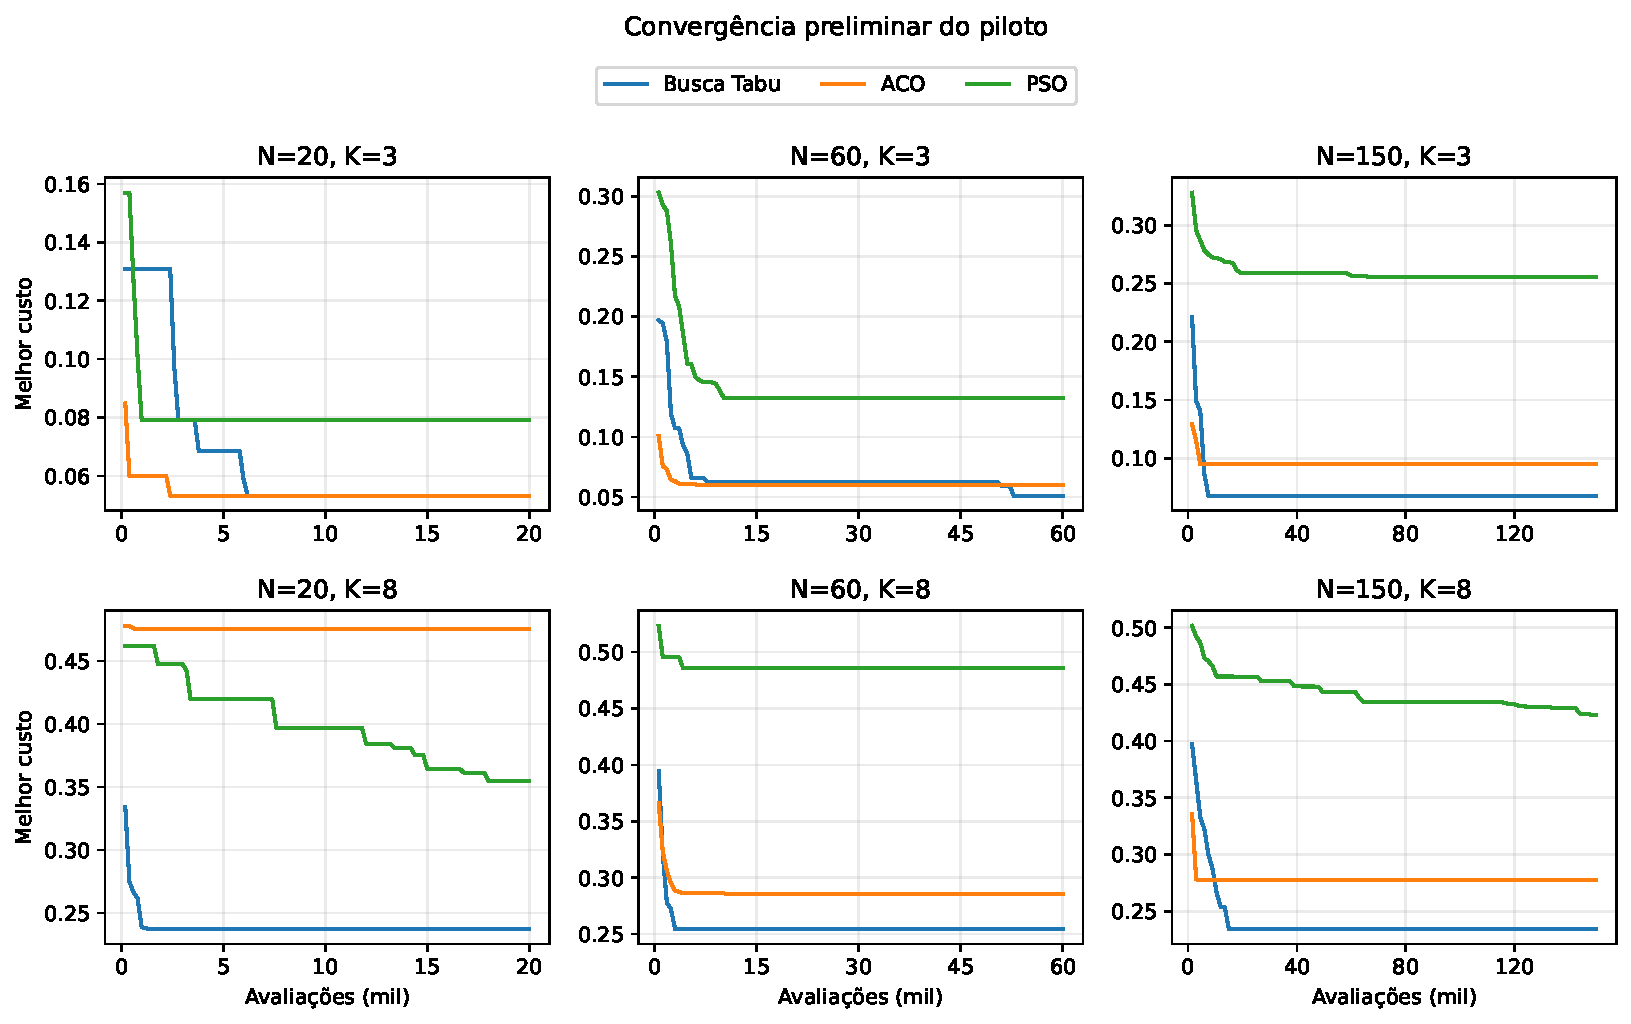
\includegraphics[width=\textwidth]{../../results/figures/pilot_convergence.pdf}
\caption{Convergência preliminar do piloto: melhor custo em função das
avaliações consumidas, por instância e por $K$.}
\label{fig:piloto-convergencia}
\end{figure}

A Figura~\ref{fig:piloto-convergencia} apresenta as curvas do piloto.

O piloto fornece uma verificação preliminar do orçamento, com uma semente por combinação
avaliada. Tomando como referência a redução de custo entre o primeiro e o último dos 100
pontos de acompanhamento, identifica-se o primeiro ponto que registra pelo menos 99,9\%
dessa redução. O primeiro ponto ocorre em 1\% do orçamento e não corresponde
necessariamente à solução inicial; a localização das melhorias tem resolução de 1\% do
orçamento. Esse indicador é retrospectivo: utiliza o resultado obtido ao término do
orçamento como referência e não estima a distância ao ótimo.

Nas execuções do ACO, o primeiro ponto que registra esse patamar ocorre entre 3\% e 18\%
do orçamento; na Busca Tabu, entre 5\% e 88\%. No PSO, há casos em que esse patamar é
atingido apenas em 90\% ou 100\% do orçamento. Melhorias próximas do limite indicam que
a estabilização não ficou demonstrada nesses casos, mas não permitem quantificar o ganho
que seria obtido com mais avaliações.

De forma análoga, um trecho final sem melhoria não demonstra que aumentar o orçamento
seria inútil. A busca pode permanecer estagnada e posteriormente alcançar outra solução.
Os orçamentos foram mantidos como condições comuns do experimento, com base na
viabilidade operacional observada no piloto, sem afirmar convergência definitiva dos
métodos ou suficiência universal do limite escolhido.

\subsubsection*{Quanto tempo custa?}

\begin{figure}[H]
\centering
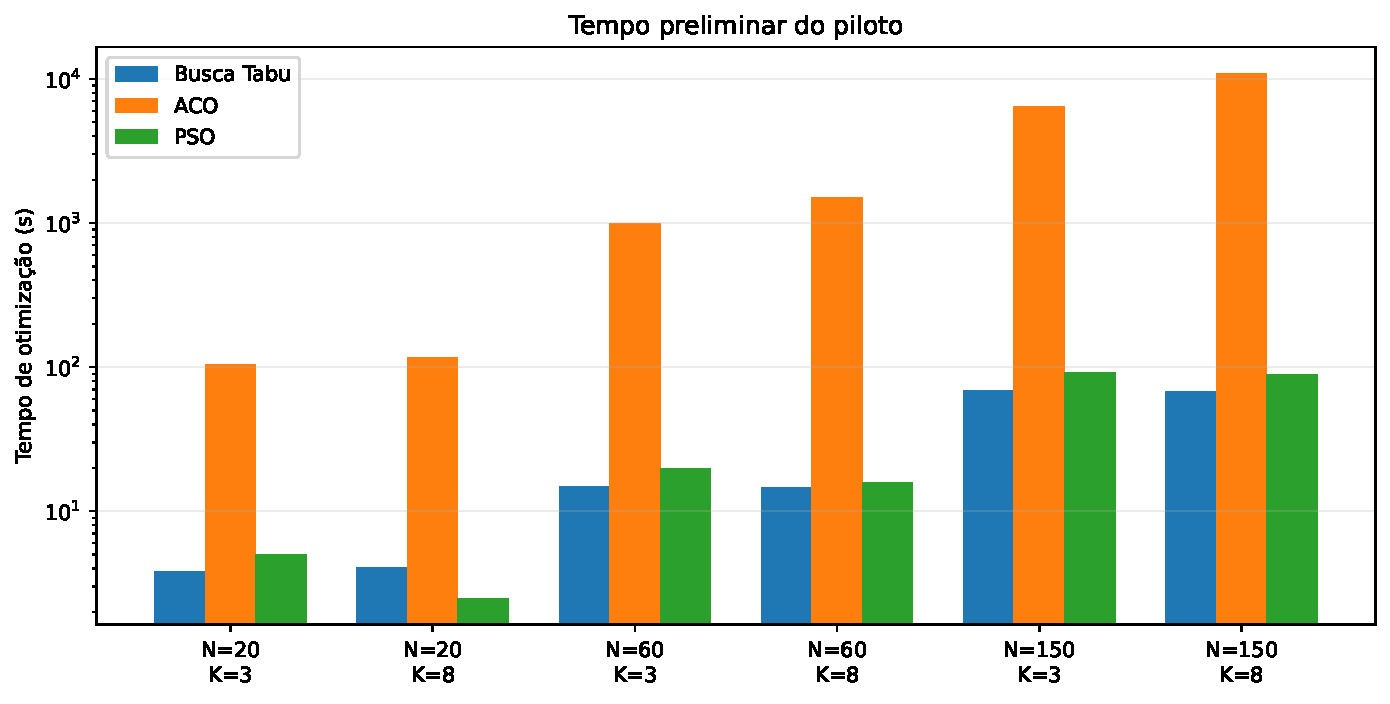
\includegraphics[width=\textwidth]{../../results/figures/pilot_time.pdf}
\caption{Tempo de otimização por cenário no piloto, em escala
logarítmica.}
\label{fig:piloto-tempo}
\end{figure}

A Figura~\ref{fig:piloto-tempo}, em escala logarítmica, mostra uma
separação de uma a duas ordens de grandeza. Na instância de 150 unidades,
a Busca Tabu completa o orçamento em cerca de $49$~s e o PSO em torno de
$70$ a $76$~s, enquanto o ACO consome de $2\,595$ a $2\,967$~s, isto é,
entre $43$ e $49$ minutos por execução. Sobre o conjunto dos seis
cenários, o ACO é de $11$ a $61$ vezes mais lento que a Busca Tabu.

A causa é estrutural e decorre da descrição da Seção~\ref{subsec:aco}: o ACO avalia o
custo parcial de cada alocação candidata a cada passo da construção de
cada formiga, de modo que o trabalho por avaliação de solução completa é
muito maior que o dos outros dois métodos, ainda que o orçamento contado
em avaliações seja idêntico. Essa medição foi o que permitiu dimensionar
a campanha oficial: com 1.620 execuções, das quais um terço em ACO, o
custo total projetado exigiu a organização em lotes e a escolha
consciente do número de \emph{workers}.

\subsubsection*{A máquina suporta o paralelismo?}

\begin{figure}[H]
\centering
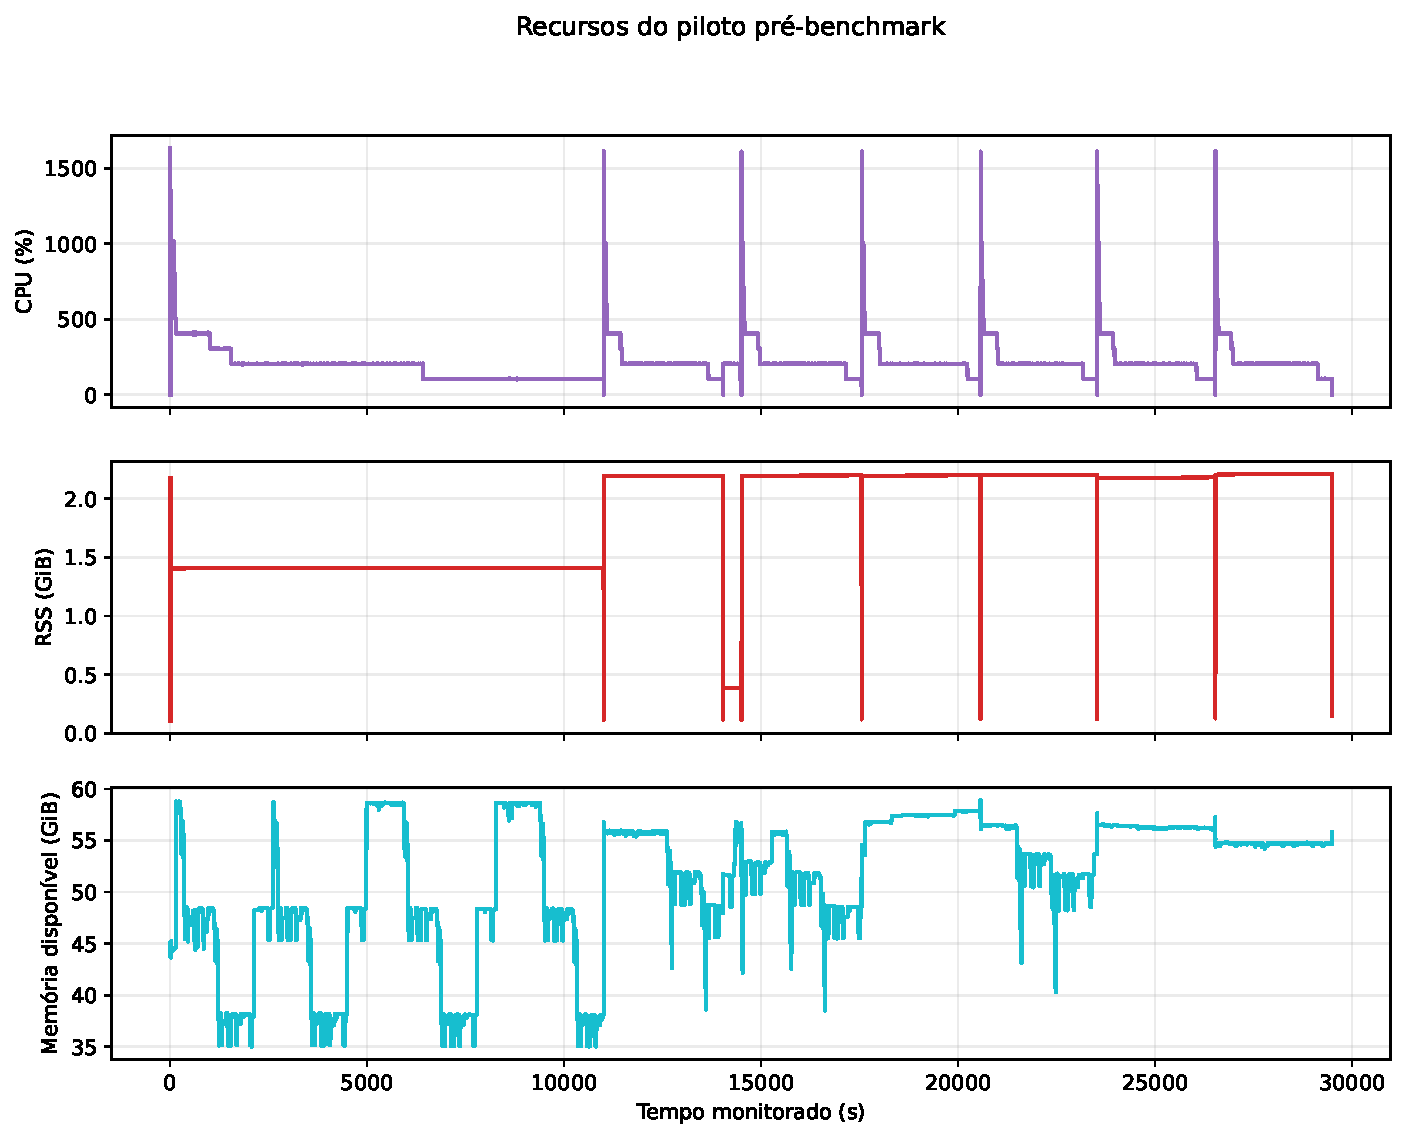
\includegraphics[width=\textwidth]{../../results/figures/pilot_resources.pdf}
\caption{Recursos consumidos durante o piloto: CPU agregada, memória
residente do processo e memória disponível do sistema.}
\label{fig:piloto-recursos}
\end{figure}

A Figura~\ref{fig:piloto-recursos} reúne 27.913 amostras coletadas em
dez sessões de monitoração. O painel superior mostra a CPU agregada
atingindo picos de $1\,635\,\%$, coerentes com os 16 \emph{workers}
configurados para os 16 núcleos físicos da máquina,
e caindo em patamares sucessivos - cerca de $400\,\%$, $200\,\%$ e
$100\,\%$ - à medida que os cenários mais curtos terminam e restam
apenas os mais longos, invariavelmente os do ACO.

O painel central mostra a memória residente estabilizada em torno de
$2{,}2$~GiB, com pico de $2{,}21$~GiB. O inferior mostra a memória
disponível do sistema oscilando entre $35$ e $59$~GiB, de um total de
$63$~GiB, sem nenhum episódio de consumo de \emph{swap}. As verificações
automáticas do monitor confirmaram, além disso, que cada otimizador
manteve uma única \emph{thread} ativa, que a CPU consumida permaneceu
dentro do limite dos \emph{workers} declarados e que nenhum processo de
otimização sobreviveu ao fim da campanha.

O monitoramento do piloto indicou condições favoráveis para operar com até 16 processos
de otimização. Esses registros apoiam o dimensionamento da campanha, mas não constituem
prova de ausência de contenção nem substituem a medição direta do tempo de CPU de cada
execução.

\subsection{Protocolo estatístico}
\label{subsec:estatistica}

A análise inferencial registrada no projeto organiza as execuções por instância, $K$ e
semente. Em cada um dos 18 cenários, aplica o teste de Friedman \cite{friedman1937} aos três algoritmos.
Quando o teste global rejeita a hipótese nula ao nível de 5\%, aplica testes bilaterais
de Wilcoxon aos três pares de algoritmos. A correção de Holm \cite{holm1979} é aplicada separadamente à
família dos três testes pareados de cada cenário. Não há correção global envolvendo os
18 testes de Friedman ou os 54 contrastes pareados do benchmark.

Os valores-p de Friedman utilizam a aproximação qui-quadrado implementada no SciPy \cite{scipyfriedman}. A
documentação recomenda cautela com essa aproximação quando há poucas amostras repetidas;
aqui são apenas três algoritmos, ainda que existam 30 sementes. Não foi realizada
calibração por permutação. Essa ressalva se refere à quantidade de algoritmos
comparados, não ao número $K$ de lotes.

O pareamento por semente é uma convenção do protocolo executado. Como os algoritmos
inicializam e consomem números pseudoaleatórios de maneiras distintas, a igualdade
numérica da semente não demonstra que as execuções estejam expostas à mesma dificuldade
aleatória. Essa limitação restringe a justificativa substantiva do pareamento e deve
acompanhar a interpretação dos valores-p. Uma análise de robustez com tratamento não
pareado seria uma extensão, não um resultado já obtido neste estudo.

O uso de testes não paramétricos dispensa a hipótese de normalidade, mas não elimina
outros pressupostos. O teste de Wilcoxon avalia a distribuição das diferenças pareadas,
com hipótese nula de simetria em torno de zero \cite{scipywilcoxon}. A aplicação registrada não inclui um
diagnóstico específico dessa simetria. Os valores-p são apresentados sob o protocolo
executado, com essas limitações explícitas.

O tamanho de efeito é expresso pela correlação bisserial de postos das diferenças de
custo, removendo diferenças exatamente nulas. Para um contraste A menos B, efeito
positivo indica custos maiores para A, portanto vantagem para B; efeito negativo indica
vantagem para A. Esse indicador resume a direção e os postos das diferenças. Sua
magnitude não mede diretamente economia financeira nem estabelece a relevância
operacional da redução de custo. Por isso, a interpretação deve considerar também as
diferenças absolutas e relativas do objetivo.

A ausência de rejeição não demonstra equivalência entre algoritmos. A comparação com a
gulosa permanece descritiva por decisão do protocolo: seu custo determinístico é tratado
como referência fixa, sem criar réplicas artificiais. Essa decisão não significa que
toda comparação inferencial com uma referência determinística seja matematicamente
impossível.

\subsection{Reprodutibilidade e pacote entregável}
\label{subsec:reproducao}

Por execução (combinação de instância, $K$, algoritmo e semente) são
registrados o custo final e o tempo de otimização (Seção~\ref{subsec:tempo}), além dos 100
checkpoints de convergência já descritos na Seção~\ref{subsec:instancias}, igualmente espaçados
ao longo do orçamento de avaliações, cada um com o melhor custo acumulado
registrado até aquele ponto. Agregando as 30 sementes de cada combinação
instância$\times K\times$algoritmo, consolidam-se as métricas de
custo médio, desvio-padrão e tempo médio, usadas em
toda a Seção~\ref{sec:resultados}.

O código, as instâncias e os resultados consolidados acompanham o repositório.
O código é distribuído sob licença MIT. Uma verificação anterior em clone
isolado confirmou a instalação pelo README e a execução da suíte automatizada.
O Apêndice~\ref{sec:guia-execucao} reúne as instruções de reprodução; as tabelas
complementares e a nova figura de distribuição são geradas por
\path{docs/relatorio/gerar_complementos.py}, a partir dos mesmos dados oficiais.

\section{Resultados e análise}
\label{sec:resultados}

\subsection{Qualidade das soluções}
\label{subsec:qualidade-solucoes}

\begin{sloppypar}
Sobre as 18 combinações instância$\times K$ do experimento principal (três
instâncias - \texttt{artesp\_rmsp\_20}, \texttt{artesp\_rmsp\_60} e
\texttt{artesp\_rmsp\_150} - combinadas com $K\in\{3,4,5,6,7,8\}$), a Busca
Tabu apresenta o menor custo médio agregado entre os três algoritmos. A média do
custo sobre as 18 combinações é $0{,}156831$ para a Busca Tabu,
contra $0{,}208578$ para o ACO e $0{,}286118$ para o PSO. Comparando
combinação a combinação, a Busca Tabu tem o menor custo médio em 17 das 18
combinações instância$\times K$.
\end{sloppypar}

A única exceção ocorre em \texttt{artesp\_rmsp\_150}, $K=5$ - a maior
instância do benchmark -, onde o ACO obtém custo médio de $0{,}156884$,
ligeiramente melhor que os $0{,}161771$ da Busca Tabu. Essa inversão de
ranking está isolada a um único cenário entre os 18, não configurando um
padrão sistemático de vantagem do ACO em instâncias grandes.

Quanto à variabilidade entre as 30 sementes de cada combinação, a Busca Tabu
também tem, em média, a menor dispersão: o desvio-padrão médio
sobre as 18 combinações é $0{,}012639$ para a Busca
Tabu, $0{,}022381$ para o ACO e $0{,}028481$ para o PSO. A Busca Tabu tem o
menor desvio-padrão em 11 das 18 combinações - uma margem mais estreita
que a observada para o custo médio, indicando que a vantagem de estabilidade
da Busca Tabu, embora presente, é menos consistente do que sua vantagem em
custo médio.

Em algumas combinações da instância pequena (\texttt{artesp\_rmsp\_20}), o
desvio-padrão da Busca Tabu chega a ser praticamente nulo - da ordem de
$10^{-17}$ a $10^{-4}$ -, indicando custos finais muito semelhantes entre sementes. Custos iguais
não demonstram, por si sós, que as partições encontradas sejam idênticas.

Os resultados completos por cenário, com melhor custo, média, desvio-padrão
amostral e tempo médio de parede, estão no Apêndice~\ref{ap:resultados}.

\begin{figure}[htbp]
\centering
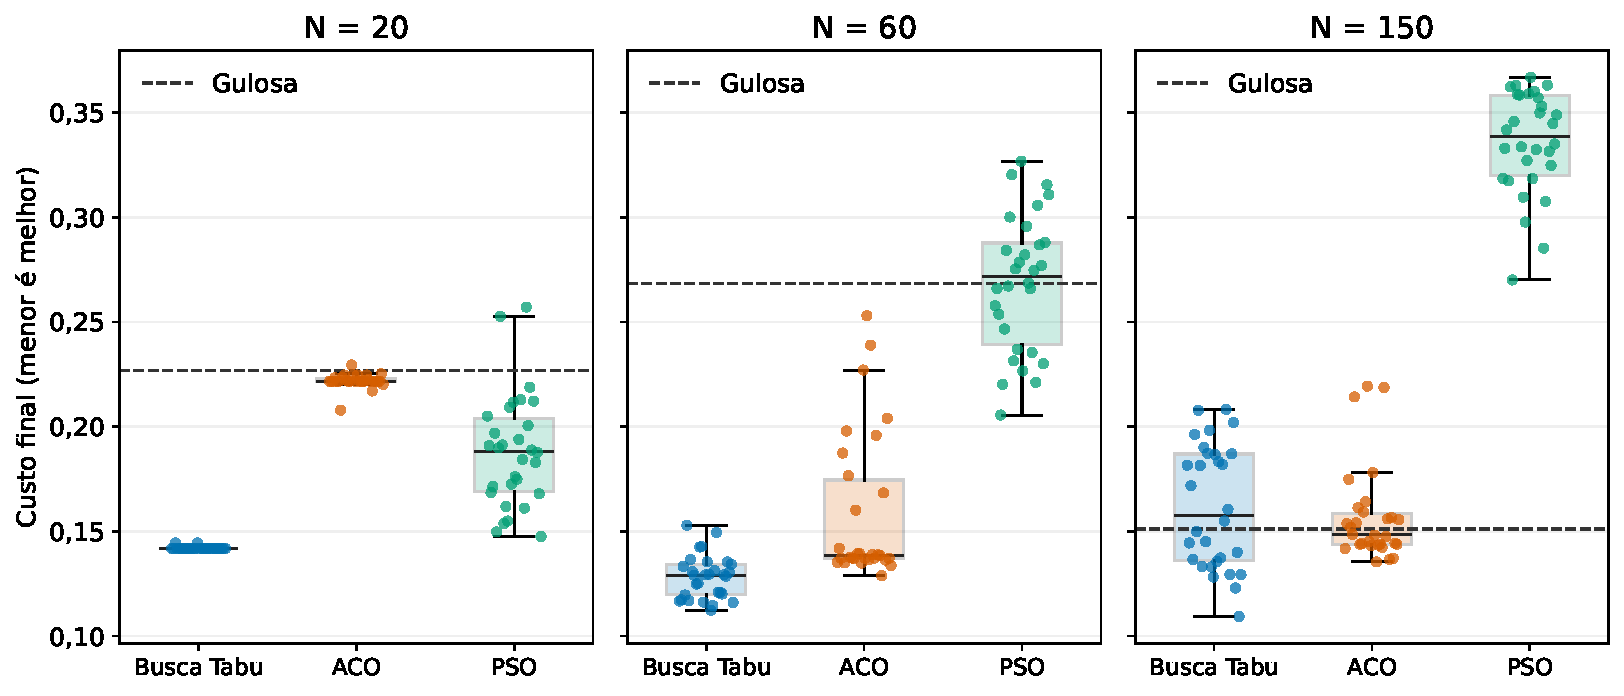
\includegraphics[width=\textwidth]{figuras/distribuicao_custos_k5.pdf}
\caption{Distribuição dos custos finais em $K=5$, com 30 execuções por
algoritmo. Cada ponto representa uma execução. As caixas vão do primeiro ao
terceiro quartil, e a linha interna é a mediana. Os bigodes alcançam os valores
observados dentro de $Q_1-1{,}5\,IQR$ e $Q_3+1{,}5\,IQR$, com $IQR=Q_3-Q_1$.
A linha tracejada indica o custo da gulosa; os painéis compartilham a escala
vertical. O deslocamento horizontal dos pontos serve apenas à legibilidade.}
\label{fig:distribuicao}
\end{figure}

\subsection{Convergência}
\label{subsec:convergencia}

As Figuras~\ref{fig:convergencia-20}, \ref{fig:convergencia-60} e
\ref{fig:convergencia-150} mostram as curvas de convergência dos três
algoritmos para $K=5$ nas três classes de tamanho de instância, com o eixo
horizontal expresso em percentual do orçamento computacional consumido.

\begin{figure}[H]
\centering
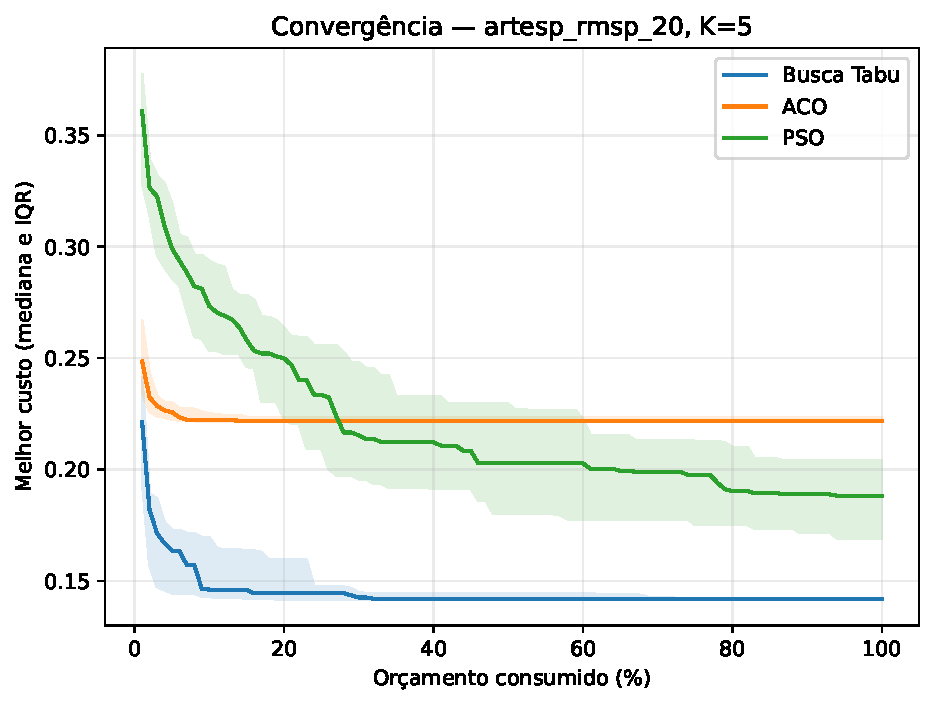
\includegraphics[width=0.8\textwidth]{../../results/figures/benchmark_convergence_20.pdf}
\caption{Curvas de convergência para \texttt{artesp\_rmsp\_20}, $K=5$.}
\label{fig:convergencia-20}
\end{figure}

\begin{figure}[H]
\centering
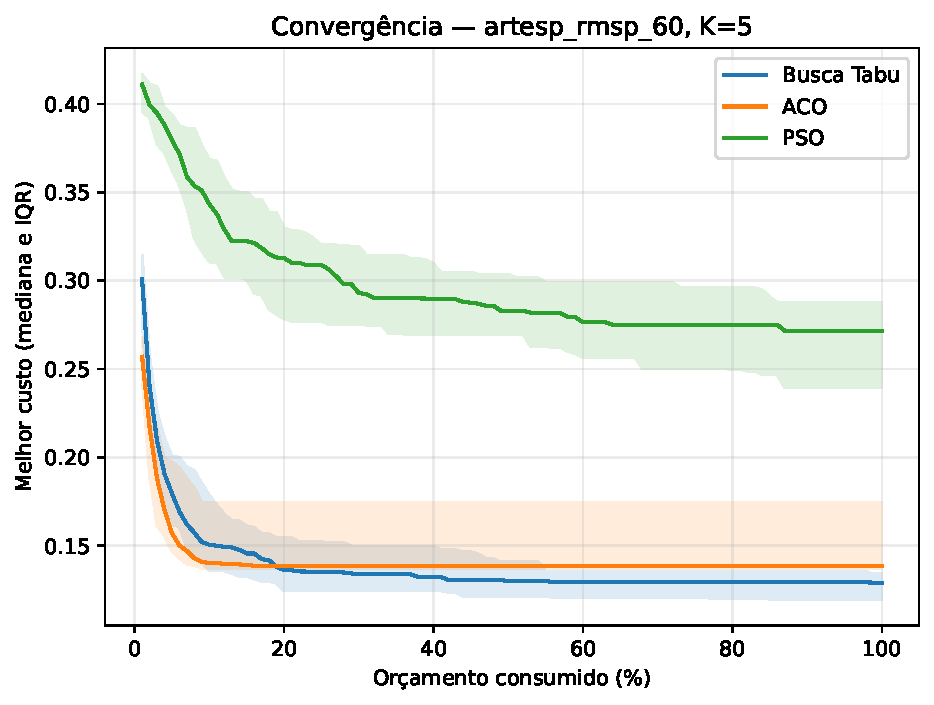
\includegraphics[width=0.8\textwidth]{../../results/figures/benchmark_convergence_60.pdf}
\caption{Curvas de convergência para \texttt{artesp\_rmsp\_60}, $K=5$.}
\label{fig:convergencia-60}
\end{figure}

\begin{figure}[H]
\centering
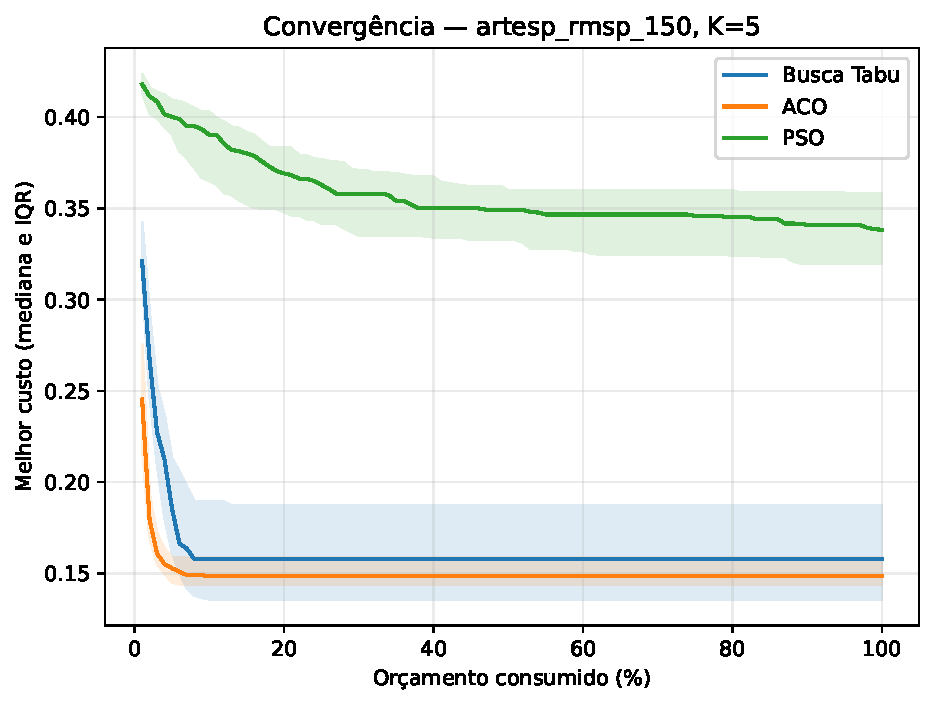
\includegraphics[width=0.8\textwidth]{../../results/figures/benchmark_convergence_150.pdf}
\caption{Curvas de convergência para \texttt{artesp\_rmsp\_150}, $K=5$.}
\label{fig:convergencia-150}
\end{figure}

O padrão que se observa nas três figuras é o de um PSO que converge mais
lentamente em relação ao seu próprio patamar final do que ACO e Busca Tabu.
Tomando como referência o primeiro checkpoint em que a mediana do custo
corrente fica a até 5\% do valor mediano final do próprio algoritmo, esse
ponto ocorre, para o PSO, entre 74\% do orçamento computacional consumido na
instância pequena (\texttt{artesp\_rmsp\_20}) e 35\% na instância grande
(\texttt{artesp\_rmsp\_150}), passando por 49\% na instância intermediária
(\texttt{artesp\_rmsp\_60}) - fração que diminui com o tamanho da instância
-, enquanto para ACO e Busca Tabu esse mesmo ponto ocorre entre 2\% e 22\%
do orçamento, em qualquer uma das três classes de tamanho.

Convergir rapidamente em relação ao próprio patamar final não implica,
porém, alcançar um patamar melhor: o ACO se aproxima do seu próprio custo
final consumindo uma fração pequena do orçamento em todas as instâncias, mas
isso não o impede de ter, na maioria das combinações, custo médio final
superior ao da Busca Tabu (Seção~\ref{subsec:qualidade-solucoes}).

\subsection{Significância estatística}
\label{subsec:significancia}

O teste de Friedman, aplicado a cada uma das 18 combinações
instância$\times K$ comparando simultaneamente PSO, Busca Tabu e ACO,
rejeita a hipótese nula $H_0$ de desempenho equivalente entre os três
algoritmos nas 18 combinações, com nível de significância $\alpha=0{,}05$.
Todos os valores-$p$ ficam abaixo de $0{,}05$, sendo o maior deles
aproximadamente $2{,}94\times10^{-7}$ (instância \texttt{artesp\_rmsp\_20},
$K=3$). A rejeição global indica diferença entre pelo menos dois algoritmos em cada
cenário, sob as aproximações e limitações da Seção~\ref{subsec:estatistica}.

Sob o protocolo inferencial executado, os contrastes do PSO com os outros dois métodos
são significativos nos 18 cenários após a correção de Holm dentro de cada cenário. Na
comparação entre Busca Tabu e ACO, não há rejeição em cinco cenários, todos na instância
de 150 unidades com $K$ de 4 a 8. Esse resultado não demonstra equivalência: indica que
o procedimento utilizado não detectou diferença nesses casos ao nível adotado.

As correlações bisseriais de postos desses cinco contrastes apresentam magnitude entre
0,0108 e 0,2731. Esses valores descrevem diferenças menos sistemáticas em postos que as
observadas nos contrastes envolvendo PSO. A relevância prática precisa ser avaliada em
conjunto com a diferença de custo e o tempo de execução. O objetivo é um índice composto
adimensional, não uma estimativa de economia operacional em moeda.

Os valores-p ajustados, efeitos com sinal e diferenças de custo médio estão no Apêndice~\ref{ap:contrastes}.

\subsection{Tempo computacional}
\label{subsec:tempo-resultados}

Sobre as 18 combinações instância$\times K$, a Busca Tabu tem o menor tempo
médio de execução entre os três algoritmos em 16
delas. A média desse tempo sobre as 18 combinações é
$20{,}05$~s para a Busca Tabu, contra $30{,}89$~s para o PSO e
$1.095{,}93$~s para o ACO. O PSO só supera a Busca Tabu por margem mínima em
duas combinações de instância pequena (\texttt{artesp\_rmsp\_20}, $K=7$ e
$K=8$), com diferenças de $0{,}007$~s e $0{,}186$~s, respectivamente.

O ACO é sistematicamente o mais lento dos três, entre cerca de ×20 e ×61
mais lento que a Busca Tabu conforme a combinação, com a construção
sequencial das formigas - e não a avaliação da função objetivo - dominando
esse custo. Em \texttt{artesp\_rmsp\_150}, $K=5$, por exemplo,
tempo médio é $2.765{,}72$~s no ACO contra $73{,}98$~s no PSO e
$48{,}73$~s na Busca Tabu. O tempo reportado é de parede, medido sob 1
thread por execução; não é uma medida de complexidade assintótica nem inclui
o custo do tuning de hiperparâmetros.

\subsection{Escalabilidade}
\label{subsec:escala}

Os fatores de crescimento do tempo entre $N=20$ e $N=150$, para $K=5$, são 22,37 para a
Busca Tabu, 24,36 para o PSO e 55,55 para o ACO. Eles descrevem o crescimento sob o
protocolo adotado, no qual o orçamento também aumenta de 20.000 para 150.000 avaliações.
Portanto, combinam o efeito de ampliar a instância, aumentar o número de avaliações e
alterar a composição dos dados. Não são estimativas de complexidade assintótica nem
isolam o custo por avaliação.

A comparação de custos entre tamanhos também exige cautela. Embora os componentes sejam
normalizados, cada instância tem unidades, distribuição de cargas e matrizes de
relacionamento próprias. Um custo menor na instância grande não prova que o algoritmo se
aproxime mais do ótimo. A comparação mais direta entre algoritmos ocorre dentro de uma
mesma instância e $K$; a comparação entre tamanhos descreve o desempenho nos três
recortes disponíveis.

\begin{figure}[H]
\centering
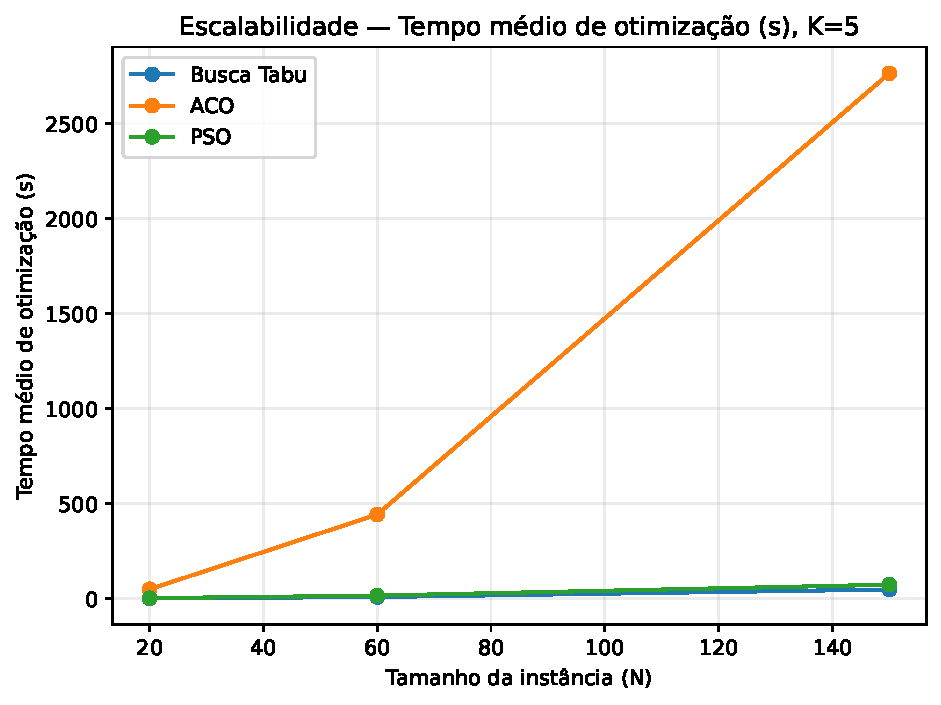
\includegraphics[width=0.8\textwidth]{../../results/figures/benchmark_scalability_time.pdf}
\caption{Tempo de execução em função do tamanho da instância, $K=5$.}
\label{fig:escalabilidade-tempo}
\end{figure}

\begin{figure}[H]
\centering
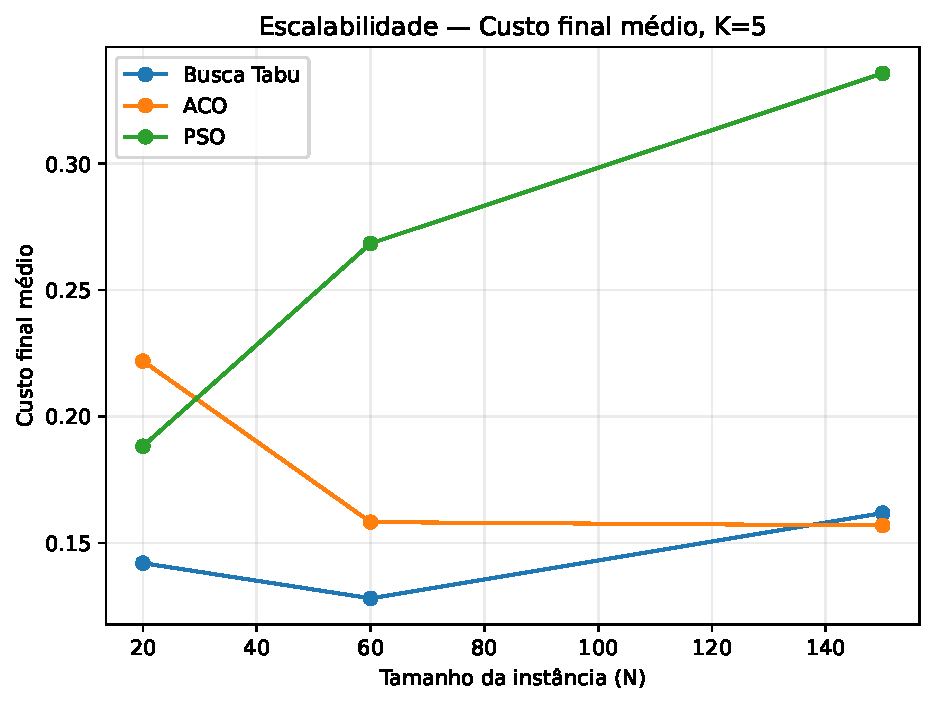
\includegraphics[width=0.8\textwidth]{../../results/figures/benchmark_scalability_quality.pdf}
\caption{Custo médio final em função do tamanho da instância, $K=5$.}
\label{fig:escalabilidade-qualidade}
\end{figure}

O custo médio final não acompanha o mesmo padrão de crescimento monótono com
o tamanho da instância que se observa para o tempo. Comparando apenas os
extremos $N=20$ e $N=150$, o ACO melhora com o aumento de $N$
($-29{,}31\%$), de forma monótona - o custo em $N=60$ fica entre os dois
extremos -, enquanto PSO ($+78{,}37\%$) e Busca Tabu ($+13{,}93\%$) pioram.
No PSO essa piora também é monótona; já na Busca Tabu não é: o custo cai em
$N=60$ (abaixo tanto de $N=20$ quanto de $N=150$) antes de voltar a subir em
$N=150$. Em termos de posição relativa entre algoritmos, o ranking geral se
mantém sem inversão ao longo do crescimento da instância, com a
exceção já registrada de \texttt{artesp\_rmsp\_150}, $K=5$, em que o ACO
supera ligeiramente a Busca Tabu (Seção~\ref{subsec:qualidade-solucoes}) -
mesmo assim, ali o tempo de execução do ACO permanece ordens de grandeza
maior que o da Busca Tabu. Não há, nestes dados, explicação causal para a
melhora de custo do ACO com o aumento de $N$; a leitura desta seção usa
apenas $K=5$ e não foi verificada nos demais valores de $K$.

\subsection{Comparação com a heurística gulosa}
\label{subsec:comparacao-gulosa}

A comparação com a heurística gulosa distingue duas perguntas: qual é a qualidade média
de uma execução estocástica e qual foi a melhor solução encontrada entre as 30
execuções. Para o primeiro critério, utiliza-se

\[
G_{\mathrm{medio}}=100\frac{C_{\mathrm{gulosa}}-\overline C_{\mathrm{meta}}}{C_{\mathrm{gulosa}}}.
\]

Valores positivos indicam menor custo médio da metaheurística. A média desse indicador
sobre os 18 cenários é 18,75\% para a Busca Tabu, -2,17\% para o ACO e -55,65\% para o
PSO. A Busca Tabu supera a gulosa em média nos 12 cenários das instâncias pequena e
média, enquanto nenhum dos três métodos o faz nos seis cenários da instância de 150
unidades.

Esse resultado não significa que todas as execuções individuais sejam piores que a
gulosa. Na instância grande, a melhor execução da Busca Tabu supera a referência nos
seis valores de $K$; a melhor execução do ACO a supera em $K=4$, 5, 6 e 7. O PSO não a
supera pelo melhor custo em nenhum desses seis cenários.

\begin{table}[htbp]
\centering\small
\caption{Comparação de média e melhor execução em $N=150$, $K=5$.}
\label{tab:gulosa-k5}
\begin{tabularx}{\textwidth}{YYYY}
\toprule
Método, $N=150$ e $K=5$ & Custo médio & Desvio-padrão amostral & Melhor custo \\
\midrule
Gulosa & 0,151036 & Não se aplica & 0,151036 \\
Busca Tabu & 0,161771 & 0,029457 & 0,109325 \\
ACO & 0,156884 & 0,022879 & 0,135396 \\
PSO & 0,335748 & 0,024647 & 0,270031 \\
\bottomrule
\end{tabularx}
\end{table}

Embora algumas execuções superem a gulosa, o conjunto das 30 execuções de cada cenário
apresenta custo médio superior ao da referência. Os ganhos individuais não se traduzem,
portanto, em vantagem média na instância grande. O melhor de 30 resultados também
utiliza um conjunto de tentativas mais amplo que uma execução individual. Portanto, sua
vantagem não deve ser apresentada como se fosse obtida pelo mesmo custo computacional de
uma única execução.

A gulosa apresenta tempos inferiores a um segundo nos cenários medidos. Assim, é uma
referência especialmente competitiva quando se priorizam rapidez e resultado
determinístico. Uma síntese descritiva adicional das execuções existentes mostra que, em
$N=150$ e $K=5$, a Busca Tabu supera a gulosa em 14 das 30 execuções, o ACO em 16 e o
PSO em nenhuma, usando tolerância de $10^{-12}$. Assim, mesmo uma maioria de execuções
melhores, como ocorre com o ACO nesse cenário, pode coexistir com custo médio superior à
referência. Essas frequências descrevem a amostra e não garantem sucesso em novas
execuções. Inicializar as metaheurísticas com a gulosa é uma extensão possível, que
exigiria um novo experimento.

As frequências de superação nos seis valores de $K$ da instância grande estão no Apêndice~\ref{ap:frequencias}.

\subsection{Análise por \texorpdfstring{$K$}{K}}
\label{subsec:k}

A Tabela~\ref{tab:k3-k8} reproduz, para $K=3$ e $K=8$, as médias sobre as
três instâncias do custo total, dos coeficientes de variação $CV_D$ e $CV_P$
e dos componentes $C_T$ e $C_A$, por algoritmo. As cinco métricas crescem,
para os três algoritmos, ao passar de $K=3$ para $K=8$.

\begin{table}[htbp]
\centering
\caption{Custo total, coeficientes de variação e componentes por algoritmo, $K=3$ e $K=8$ (médias sobre as três instâncias).}
\label{tab:k3-k8}
\begin{tabular}{lrrrrr}
\toprule
Algoritmo & Custo total & $CV_D$ & $CV_P$ & $C_T$ & $C_A$ \\
\midrule
\multicolumn{6}{l}{\textit{$K=3$}} \\
ACO & 0,0712 & 0,0413 & 0,0899 & 0,0653 & 0,1008 \\
PSO & 0,1490 & 0,0588 & 0,0417 & 0,2272 & 0,2785 \\
Busca Tabu & 0,0628 & 0,0447 & 0,0556 & 0,0643 & 0,0951 \\
\midrule
\multicolumn{6}{l}{\textit{$K=8$}} \\
ACO & 0,3413 & 0,7418 & 0,7271 & 0,2341 & 0,3175 \\
PSO & 0,4174 & 0,3088 & 0,2665 & 0,5860 & 0,6933 \\
Busca Tabu & 0,2404 & 0,3178 & 0,2513 & 0,2510 & 0,3474 \\
\bottomrule
\end{tabular}
\end{table}

Aumentar o número de lotes de 3 para 8 piora, em média, todas as métricas
medidas para os três algoritmos - não há, nestes dados, nenhum valor de $K$
que reduza simultaneamente todas as cinco métricas em relação a valores
de $K$ menores. O ACO é o mais sensível ao aumento de $K$ em $CV_D$ e
$CV_P$ (razão $K{=}8/K{=}3$ de cerca de dezoito e oito vezes,
respectivamente). Em termos de crescimento absoluto de custo total, a Busca
Tabu tem o menor aumento entre os três ($+0{,}1776$, contra $+0{,}2701$ no
ACO e $+0{,}2683$ no PSO); em termos de razão $K{=}8/K{=}3$, porém, é o PSO
que cresce menos (×2,80, contra ×3,83 na Busca Tabu e ×4,79 no ACO) - as
duas leituras, absoluta e relativa, não apontam para o mesmo algoritmo.

Estendendo essa leitura aos seis valores de $K$, o crescimento é monótono ou
quase monótono para os três algoritmos, com uma única exceção identificada:
a Busca Tabu em $CV_P$, que cai de $K=3$ para $K=4$ antes de voltar a
crescer a partir de $K=5$. Por decisão metodológica registrada no protocolo
experimental do projeto, este relatório não declara um valor de $K$ ótimo,
relatando apenas ganhos marginais e possíveis compromissos entre os cinco
indicadores. Nesse sentido, os dados não
mostram, na faixa $K\in\{3,\ldots,8\}$ testada, um ponto em que mais lotes
melhorem coerência territorial ou funcional às custas de equilíbrio, ou
vice-versa - as duas famílias de métrica pioram juntas, o que caracteriza
um compromisso a ser resolvido por critérios institucionais e não por um
ótimo automático desta formulação.

\subsection{Sensibilidade a hiperparâmetros}
\label{subsec:sensibilidade}

As médias marginais por nível descrevem a sensibilidade dentro dessa grade. Por se
tratar de uma grade fatorial, cada nível é observado em combinação com os demais
fatores; a síntese marginal não demonstra que o efeito seja uniforme entre combinações
nem descreve interações entre parâmetros. Os resultados não serão apresentados como
prova de que apenas um parâmetro explica o comportamento do algoritmo.

Na grade avaliada, o parâmetro com maior diferença marginal do ACO é \texttt{alpha}: a
diferença de custo médio entre seus dois níveis testados
($0{,}1342$) é cerca de três vezes a do segundo parâmetro mais influente do
próprio ACO (\texttt{beta}, $0{,}0434$) e entre nove e cinquenta vezes maior
que a de qualquer parâmetro individual de PSO ou Busca Tabu. No PSO, os
quatro parâmetros têm efeito comparativamente pequeno e semelhante entre si,
em ordem crescente de sensibilidade: \texttt{n\_particles}, \texttt{cognitive},
\texttt{social} e \texttt{inertia}. Na Busca Tabu, as diferenças entre
níveis são as menores das três metaheurísticas, e o parâmetro mais sensível
é \texttt{tabu\_tenure}, cujo efeito não é monótono: o menor custo médio
ocorre no nível intermediário (tenure$=10$), não nos extremos testados
(tenure$=5$ ou tenure$=20$).

\subsection{Aceleração por GPU}
\label{subsec:gpu}

O estudo adicional transfere a avaliação em lote da função objetivo à GPU e mantém as
demais etapas no processador. A cobertura é restrita a $N=150$ e $K=5$: 30 execuções do
PSO e três do ACO. A aceleração é calculada como razão entre o tempo da execução em CPU
e o da execução em GPU de mesma semente. A média dessas razões para o PSO é 1,814, com
desvio-padrão amostral de 0,078 e valores de 1,520 a 1,974; os três casos do ACO ficam
entre 1,002 e 1,026.

Para o PSO, a fração de aproximadamente 46\% do tempo atribuída à avaliação fornece,
pela lei de Amdahl \cite{amdahl1967}, uma referência idealizada de $1/(1-0{,}46)$, aproximadamente 1,852. A
proximidade da média observada a esse valor é compatível com o perfilamento, mas não
demonstra que cada execução esteja limitada pelo mesmo número. A fração é aproximada e
tempos variam entre execuções; de fato, alguns valores individuais superam essa
referência. Não se atribui a diferença residual exclusivamente a transferências ou
lançamento de kernels sem decomposição suficiente para demonstrá-lo.

No perfilamento do ACO, a construção sequencial concentra aproximadamente 98,7\% do
tempo de uma geração. Essa etapa permanece no processador no desenho avaliado, o que
limita o ganho de acelerar apenas a avaliação final em lote. As decisões de uma mesma
formiga dependem do estado parcial anterior; isso não implica impossibilidade de
paralelizar formigas independentes em outro desenho. O resultado obtido caracteriza esta
implementação híbrida e os três casos medidos, não todos os usos de ACO em GPU.

\section{Análise espacial dos agrupamentos}
\label{sec:analise-espacial}

Os indicadores agregados descrevem equilíbrio e relações cortadas, mas não mostram
diretamente a distribuição dos lotes no território. A análise cartográfica examina as
imagens apresentadas para os três algoritmos na instância de 150 unidades com $K=5$. O
recorte é ilustrativo: não representa a variabilidade entre as 30 execuções nem permite
estender automaticamente o padrão visual aos demais cenários. O manifesto de exportação
identifica separadamente as melhores soluções selecionadas, cujas sementes e custos são
apresentados na tabela de apoio.

No processo de exportação, os rótulos são alinhados por máxima sobreposição de unidades
em relação à solução de referência. O alinhamento remove a arbitrariedade dos nomes dos
lotes, sem tornar os grupos idênticos. A associação entre cores de imagens diferentes
depende de elas terem sido produzidas com esse mesmo alinhamento. A leitura qualitativa
de concentração e mistura de cores dentro de cada imagem independe de conhecer o nome
atribuído a cada lote.

O manifesto identifica as soluções exportadas, mas os PNG incluídos não
registram semente, custo ou identificador que comprovem essa correspondência.
Por isso, a interpretação das imagens é qualitativa. As soluções identificadas
no manifesto são descritas separadamente no Apêndice~\ref{ap:lotes}.

\begin{figure}[H]
  \centering
  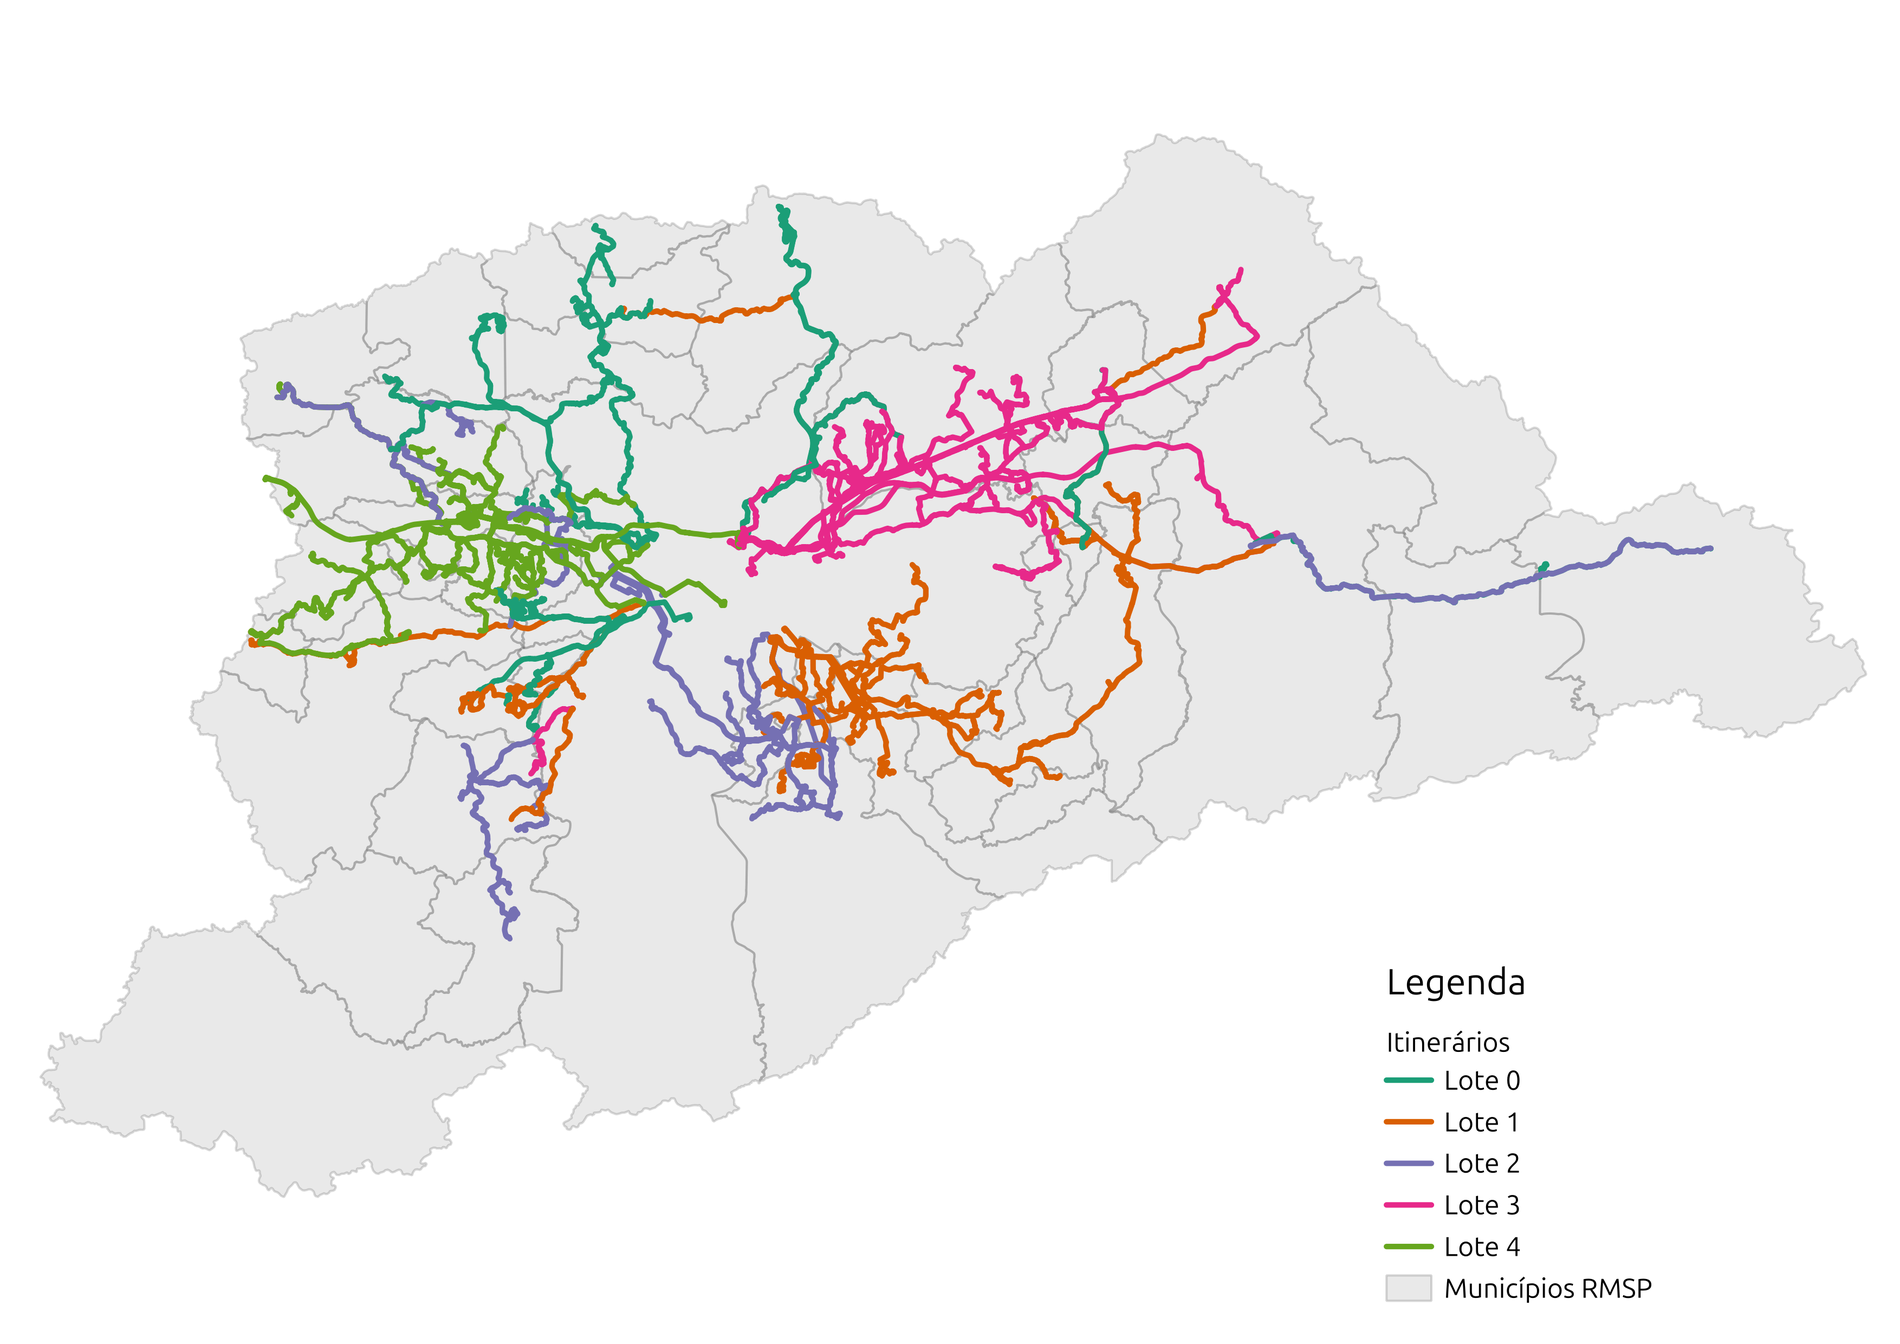
\includegraphics[width=\textwidth]{figuras/mapa_tabu_k5.png}
  \caption{Distribuição dos itinerários por lote na solução ilustrada da Busca Tabu, para 150 unidades e $K=5$. A concentração visual de cores não demonstra conectividade ou compacidade.}
  \label{fig:mapa-tabu}
\end{figure}

\begin{figure}[H]
  \centering
  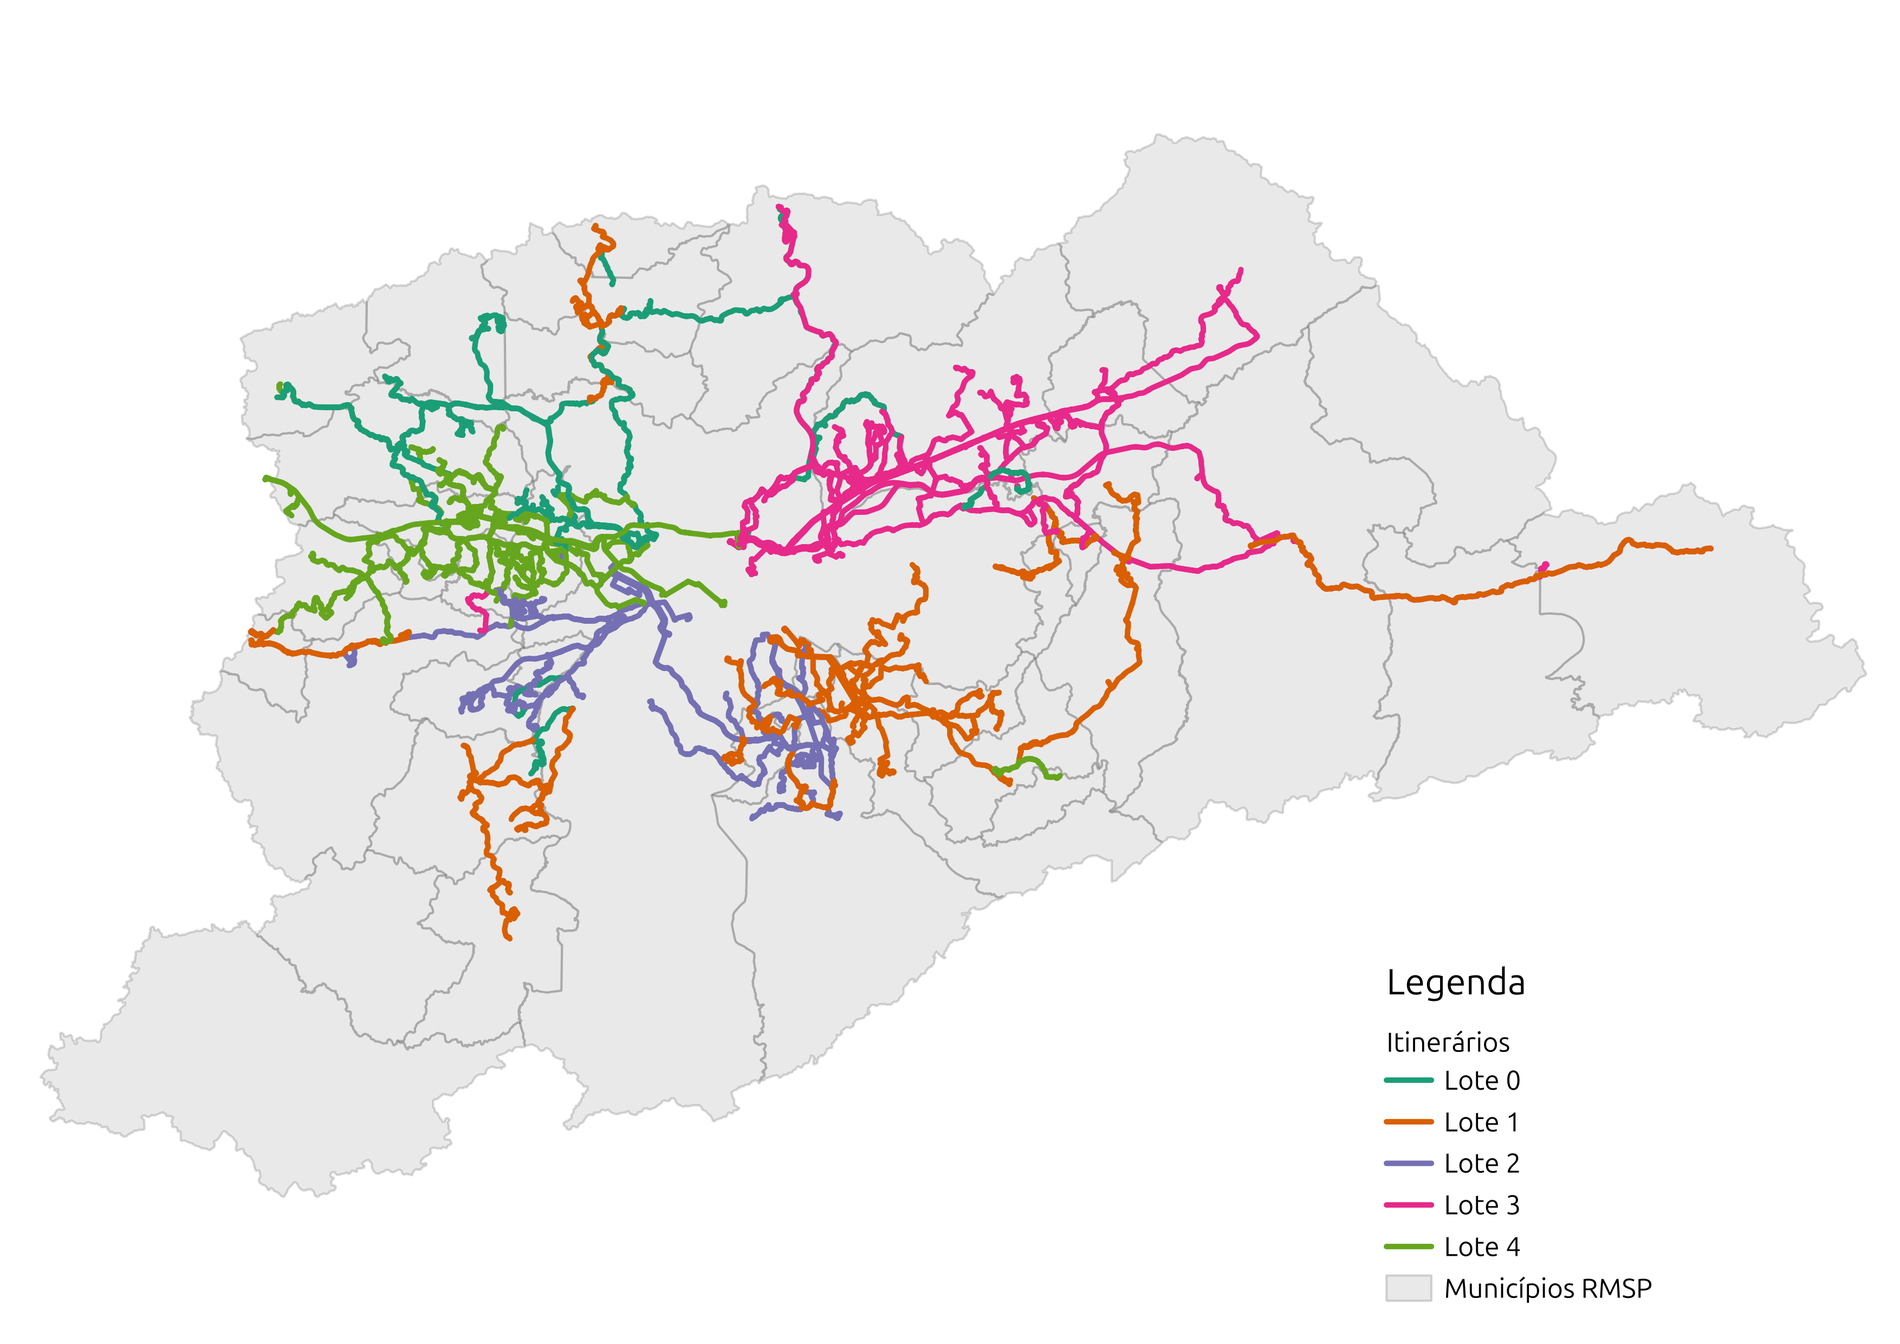
\includegraphics[width=\textwidth]{figuras/mapa_aco_k5.png}
  \caption{Distribuição dos itinerários por lote na solução ilustrada do ACO, para 150 unidades e $K=5$. A interpretação é qualitativa e se refere à execução representada.}
  \label{fig:mapa-aco}
\end{figure}

\begin{figure}[H]
  \centering
  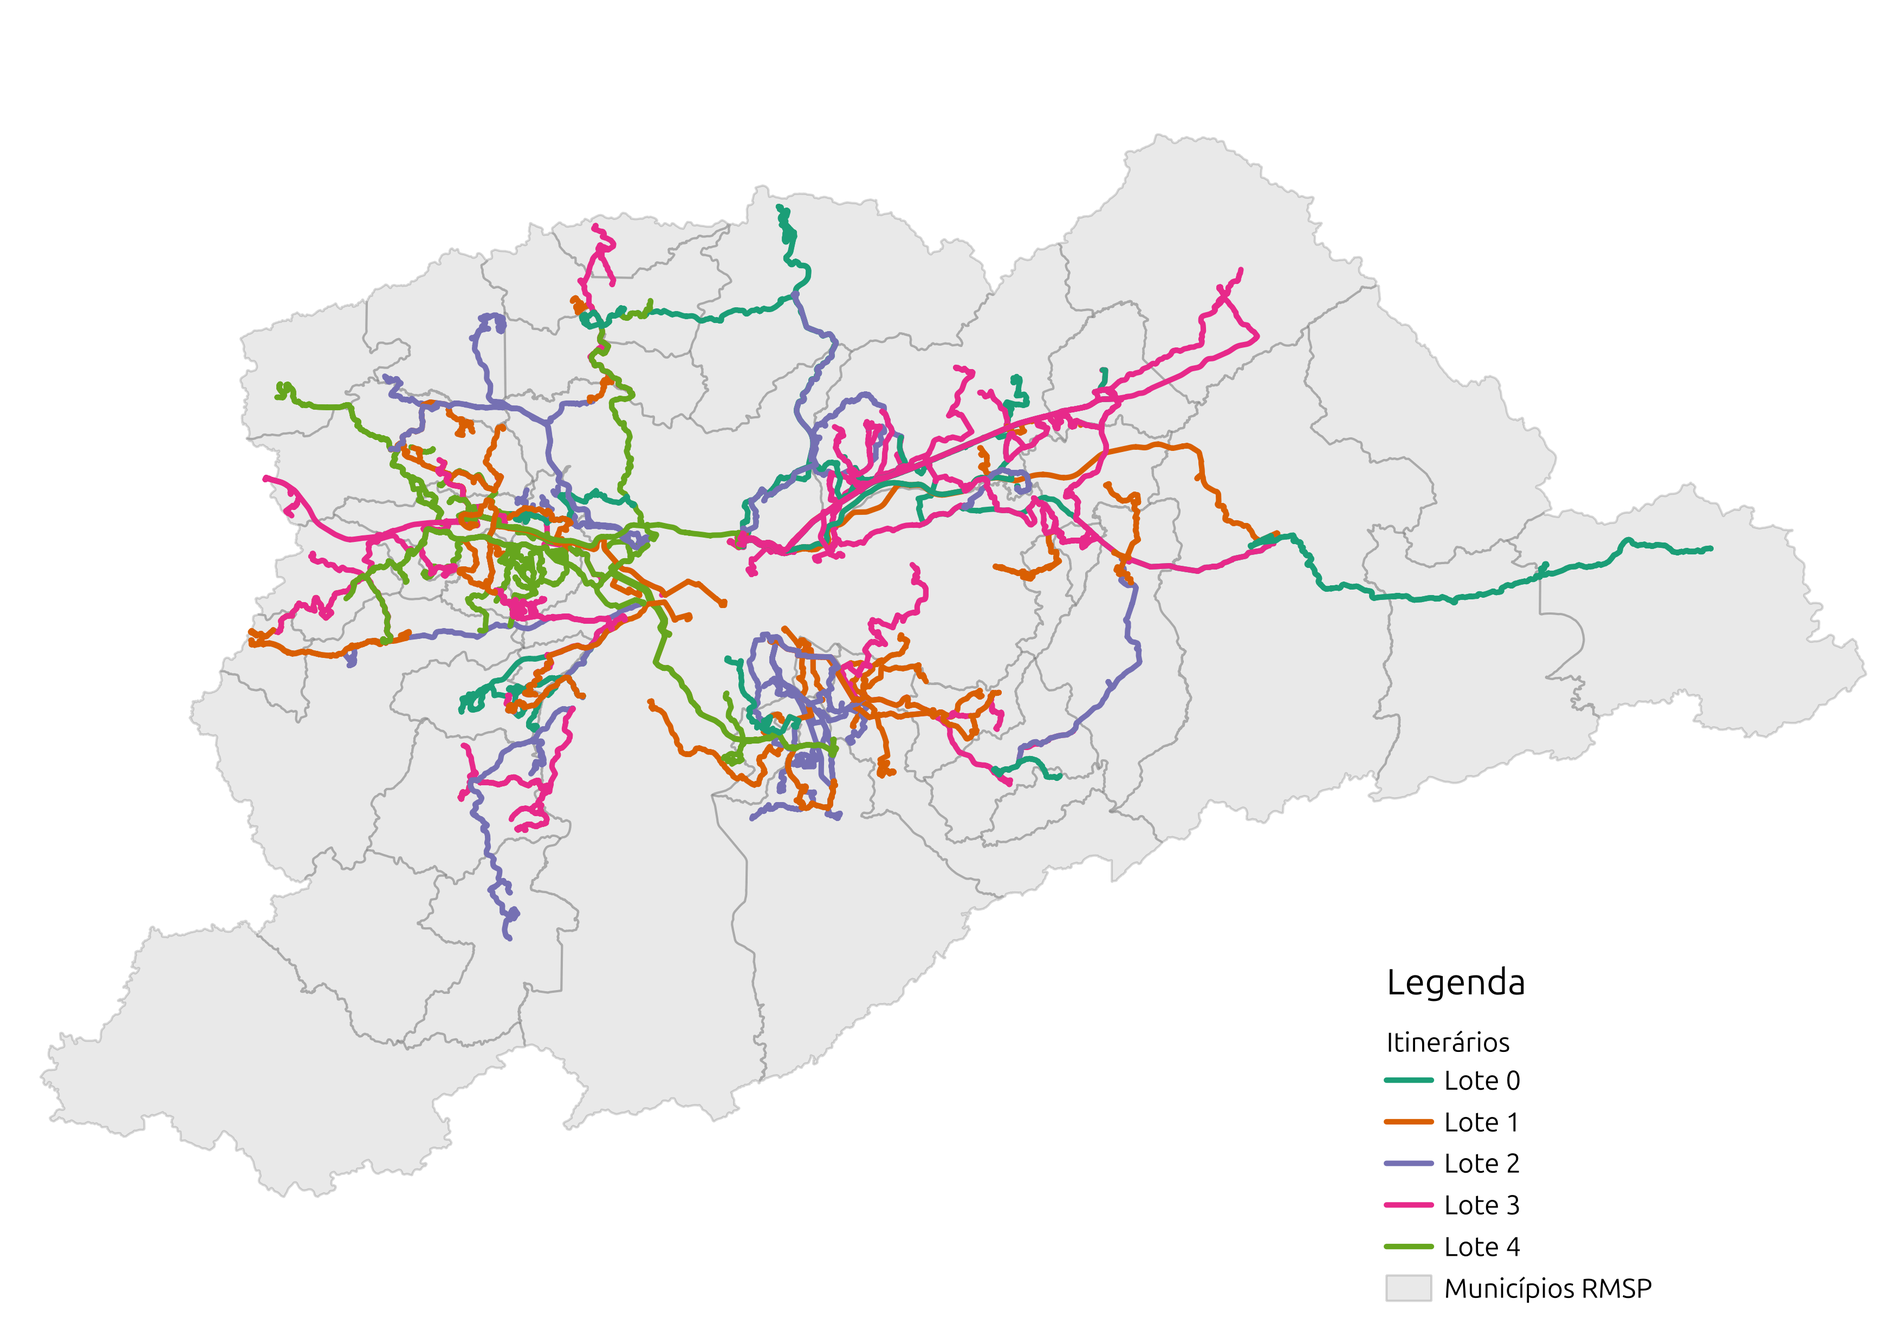
\includegraphics[width=\textwidth]{figuras/mapa_pso_k5.png}
  \caption{Distribuição dos itinerários por lote na solução ilustrada do PSO, para 150 unidades e $K=5$. A mistura de cores permite examinar a separação de itinerários em áreas comuns.}
  \label{fig:mapa-pso}
\end{figure}

\subsection{Leitura visual e implicações operacionais}

Nas soluções ilustradas, Busca Tabu e ACO apresentam concentrações territoriais
visualmente mais reconhecíveis, enquanto o PSO mostra maior mistura de cores em áreas
comuns. Essa leitura é qualitativa. Coesão visual, conectividade e compacidade são
propriedades distintas, e o modelo não impõe uma restrição explícita que garanta as duas
últimas.

Se os lotes forem atribuídos a operadores diferentes, a presença de vários operadores em
um mesmo território poderá implicar maior necessidade de coordenação. Entretanto, o
experimento não mede custos fixos, fiscalização ou reorganização da rede. Portanto, as
figuras não demonstram, por si sós, aumento de custo operacional nem inviabilidade
administrativa das soluções.

\subsection{Mecanismos compatíveis com os padrões observados}

Os três algoritmos avaliam a mesma função objetivo, mas incorporam essa informação em
decisões diferentes. Na Busca Tabu, cada candidato realoca uma unidade, e seu custo
permite comparar diretamente as alternativas amostradas. A decisão utiliza o custo
total: um aumento do componente territorial pode ser compensado por reduções de
desequilíbrio ou de afinidade cortada. Além disso, a busca pode aceitar piora no custo
total quando esse é o melhor movimento admissível.

No ACO, os custos parciais orientam a atribuição de cada unidade aos lotes permitidos. A
heurística considera as relações com as unidades já alocadas; o feromônio reforça
atribuições presentes em boas soluções completas. Essa construção usa informação local
sobre as alternativas, sem demonstrar que o efeito de uma decisão seja independente das
demais.

No PSO, cada chave é decodificada em uma faixa de lote. A atualização contínua é
orientada pelos melhores estados pessoal e global, que refletem indiretamente todos os
componentes da função objetivo. O reparo também consulta o custo das realocações
candidatas. Portanto, a informação territorial não está ausente do PSO, embora o
operador de velocidade não utilize explicitamente a matriz de afinidade para decidir
cada movimento de unidade.

A diferença de acesso à informação local é uma hipótese compatível com o padrão espacial
encontrado. O experimento não a isola das demais diferenças de inicialização,
representação, memória e uso do orçamento. Atribuir causalidade exigiria comparar
variantes controladas, por exemplo com e sem um operador de refinamento territorial,
preservando as demais condições.

\subsection{Unidades com poucas relações territoriais}

O componente territorial penaliza a massa de sobreposição cortada entre lotes. Por isso,
unidades com pequena soma de relações territoriais exercem influência limitada sobre
esse componente, mesmo quando ficam afastadas da concentração principal do lote.

Para a matriz territorial simétrica e não negativa, definindo \(s_i=\sum_{j\ne
i}S_{ij}\) e \(M=\sum_{i<j}S_{ij}>0\), uma realocação isolada da unidade i que preserve
os $K$ lotes ativos satisfaz

\[
|\Delta C_T|\leq \frac{s_i}{M}.
\]

Isso ocorre porque apenas os pares incidentes em i podem mudar de situação, e sua massa
total é \(s_i\). Para \(M=0\), o componente territorial é zero por definição. A
desigualdade descreve a sensibilidade de um componente da função, não a qualidade final
da solução ou a dinâmica completa da busca.

Uma pequena massa territorial não torna a alocação indiferente para o objetivo completo.
O componente funcional também depende das relações incidentes na unidade, e os
componentes de demanda e produção respondem à sua transferência. Assim, a ocorrência de
linhas afastadas é compatível com uma limitação do critério territorial adotado, mas não
permite excluir influência dos demais componentes ou insuficiência da busca.

Na instância de 150 unidades, a mediana da massa territorial incidente por unidade é
2,781. As quinze unidades com menor massa reúnem 1,58\% da soma das massas incidentes de
todas as unidades, na qual cada par é contado duas vezes. A menor massa é 0,0813,
aproximadamente 2,92\% da mediana. Essas estatísticas foram recalculadas a partir da
matriz territorial da instância versionada.

\subsection{Garagens e oficinas}

A localização de garagens e oficinas é uma dimensão operacional não representada na
formulação. Os dados necessários não foram incorporados ao estudo; portanto, o modelo
não calcula percursos sem passageiros entre bases e itinerários nem verifica capacidade
ou disponibilidade dessas instalações.

Uma solução com baixo custo no objetivo adotado não constitui, por isso, uma
demonstração de viabilidade operacional de uma concessão ou de um arranjo real de
operadores. Acrescentar distância a bases, capacidade de atendimento ou uma medida de
compacidade seria uma extensão da formulação. Cada termo exigiria dados, interpretação
operacional, normalização e nova comparação dos algoritmos.

\section{Discussão e conclusões}
\label{sec:conclusoes}

Entre as três metaheurísticas avaliadas, a Busca Tabu apresenta a combinação mais
favorável de qualidade média e tempo de parede: alcança o menor custo médio em 17 dos 18
cenários e o menor tempo médio em 16. Essa conclusão se refere às implementações,
parâmetros congelados e limites de avaliação deste estudo, sem estabelecer superioridade
geral da Busca Tabu em problemas de transporte.

A inclusão da heurística gulosa modifica a recomendação prática. Na instância grande,
seu custo é inferior à média das três metaheurísticas, com tempo muito menor. A Busca
Tabu, entretanto, encontra soluções individuais melhores nos seis valores de $K$, e o
ACO em quatro. Assim, a escolha depende de privilegiar uma solução rápida e
determinística ou aceitar o custo de múltiplas tentativas em busca de soluções melhores.
A vantagem do melhor resultado observado deve ser ponderada pelo custo de realizar e
selecionar essas tentativas.

A adaptação do PSO exige compatibilizar atualizações contínuas com a partição discreta.
A decodificação, o reparo quando necessário e a projeção mantêm a coerência entre
estados contínuo e discreto, mas introduzem trabalho adicional. Os experimentos não
isolam quanto cada mecanismo contribui para o desempenho final. Seu ganho com GPU reduz
tempo no recorte medido, sem demonstrar melhora na qualidade da solução.

No ACO, o custo da construção orientada por avaliações parciais explica uma parcela
substancial do esforço computacional observado. A pequena aceleração no desenho híbrido
acompanha o fato de que essa etapa permanece no processador. O estudo adicional não
inclui Busca Tabu e não cobre outros tamanhos ou valores de $K$.

A análise cartográfica complementa os indicadores e evidencia que penalizar relações
cortadas não garante lotes compactos ou viabilidade de atendimento a partir de garagens.
As extensões prioritárias são examinar a robustez aos pesos e às aproximações dos dados,
testar inicialização pela gulosa e estudar medidas explícitas de distância ou acesso a
bases operacionais. Mudanças de formulação ou de algoritmo exigiriam nova comparação
experimental. O número de lotes permanece externo ao modelo; os resultados não
fundamentam uma recomendação institucional de $K$ ótimo.

\subsection{Limitações e extensões futuras}

O estudo utiliza uma instância por tamanho, proveniente de uma única rede,
e parâmetros ajustados apenas em $N=60$, $K=5$. O orçamento cresce com $N$,
de modo que a escalabilidade observada combina ampliação da instância e maior
número de avaliações. O tempo consolidado é de parede; a medida de CPU
solicitada pelo enunciado não foi obtida na mesma janela por execução.
As inferências seguem o pareamento por semente e as aproximações estatísticas
descritas na Seção~\ref{subsec:estatistica}. Essas limitações restringem a
generalização dos resultados.

Os pesos iguais e os raios de 200~m para sobreposição e 400~m para acesso
e transferências são hipóteses fixadas pelo projeto. Estudos de sensibilidade
poderiam verificar sua influência sobre o ranking. Outra extensão é retirar
a similaridade de mercados O-D e renormalizar a afinidade, distinguindo sua
contribuição das relações de terminal e integração potencial. A inclusão de
garagens, medidas de compacidade e custos institucionais de $K$ exige dados
adicionais e uma nova formulação, sem modificar retroativamente o benchmark
apresentado.

\clearpage
\phantomsection
\addcontentsline{toc}{section}{Referências}
\bibliographystyle{plain}
\bibliography{referencias}

\clearpage
\appendix
% Gerado por docs/relatorio/gerar_complementos.py; não editar as tabelas manualmente.

% Fonte: results/tables/benchmark_runs.parquet; SHA256: 362b73efe890dc115e73ee12cd1c9c8b5b4c06ae858d947bb2191ae84a7ca93f

% Fonte: results/tables/benchmark_summary.parquet; SHA256: 107f507f19ea58c837ce75098c0db7240953509c719478e4b8167eff2ce8240d

% Fonte: results/tables/greedy_runs.parquet; SHA256: f7d3f4d60086058baebbd6940d1411d0d7b87c18038bfeb644eb3c2e24b6dec4

% Fonte: results/tables/benchmark_statistical_tests.parquet; SHA256: 9b8122b875897e136d547a3f88c72571a7ed72f9d55dbde1500b2bff4a6f9e6f

% Fonte: results/maps/lot_maps_manifest.json; SHA256: 258acec2ca1f5cb19a169f6b7b70e90bb9d62cc4a7a86f9a26ff1b42984ade38

% Fonte: data/instances/artesp_rmsp_150.json; SHA256: 7ab22bad2ea9669a1fc1205e2ba2f1cf6af4d608c2ce5a2e2b6cb474c072be5d

% Fonte: data/instances/artesp_rmsp_150_units.parquet; SHA256: 8c4bd3cb5b1367259406cadfe36bf6654f1d230a7383604d346863ae6eaeb617

% Fonte: data/instances/artesp_rmsp_150_pair_metrics.parquet; SHA256: 4bf5b7b1b68bac594a1aab6b0b47119dfd7ccf7b48eca89f26c0f095a1ebc2cd

\section{Resultados completos por cenário}\label{ap:resultados}

Média, desvio-padrão amostral (DP) e melhor custo das 30 execuções de cada cenário. O tempo é a média do tempo de parede de uma execução, em segundos. O melhor de 30 resultados não representa o esforço de uma tentativa única. As tabelas são extraídas dos resultados oficiais, sem novas execuções. Valores exibidos são arredondados; as comparações usam os números completos.

\begingroup\small
\setlength{\tabcolsep}{5pt}
\begin{longtable}{rlrrrr}
\caption{Resultados da instância de 20 unidades.}\label{tab:resultados-20}\\
\toprule
$K$ & Algoritmo & Custo médio & DP & Melhor custo & Tempo (s) \\
\midrule
\endfirsthead
\multicolumn{6}{c}{\tablename~\thetable{} (continuação)}\\
\toprule
$K$ & Algoritmo & Custo médio & DP & Melhor custo & Tempo (s) \\
\midrule
\endhead
\midrule\multicolumn{6}{r}{Continua na próxima página}\\
\endfoot
\bottomrule
\endlastfoot
3 & Busca Tabu & 0,053567 & 0,004054 & 0,052082 & 2,17 \\
3 & ACO & 0,054689 & 0,004032 & 0,053244 & 47,26 \\
3 & PSO & 0,072698 & 0,014452 & 0,052082 & 4,02 \\
4 & Busca Tabu & 0,085926 & 0,001080 & 0,085520 & 2,16 \\
4 & ACO & 0,151439 & 0,022184 & 0,103257 & 48,52 \\
4 & PSO & 0,109686 & 0,020028 & 0,085520 & 3,52 \\
5 & Busca Tabu & 0,141994 & 0,000670 & 0,141814 & 2,18 \\
5 & ACO & 0,221928 & 0,003362 & 0,207856 & 49,79 \\
5 & PSO & 0,188231 & 0,026990 & 0,147567 & 3,04 \\
6 & Busca Tabu & 0,182745 & 0,000077 & 0,182725 & 2,18 \\
6 & ACO & 0,293670 & 0,017588 & 0,254001 & 48,22 \\
6 & PSO & 0,253155 & 0,030507 & 0,197295 & 2,44 \\
7 & Busca Tabu & 0,214347 & 0,000000 & 0,214347 & 2,19 \\
7 & ACO & 0,379521 & 0,023039 & 0,315987 & 45,81 \\
7 & PSO & 0,308183 & 0,030370 & 0,256408 & 2,18 \\
8 & Busca Tabu & 0,237502 & 0,000000 & 0,237502 & 2,19 \\
8 & ACO & 0,448785 & 0,029295 & 0,342081 & 43,44 \\
8 & PSO & 0,359115 & 0,028553 & 0,289573 & 2,01 \\
\end{longtable}
\endgroup

\begingroup\small
\setlength{\tabcolsep}{5pt}
\begin{longtable}{rlrrrr}
\caption{Resultados da instância de 60 unidades.}\label{tab:resultados-60}\\
\toprule
$K$ & Algoritmo & Custo médio & DP & Melhor custo & Tempo (s) \\
\midrule
\endfirsthead
\multicolumn{6}{c}{\tablename~\thetable{} (continuação)}\\
\toprule
$K$ & Algoritmo & Custo médio & DP & Melhor custo & Tempo (s) \\
\midrule
\endhead
\midrule\multicolumn{6}{r}{Continua na próxima página}\\
\endfoot
\bottomrule
\endlastfoot
3 & Busca Tabu & 0,053257 & 0,003080 & 0,047411 & 9,08 \\
3 & ACO & 0,068253 & 0,015180 & 0,054883 & 416,11 \\
3 & PSO & 0,151270 & 0,035280 & 0,088751 & 15,51 \\
4 & Busca Tabu & 0,088016 & 0,010192 & 0,074024 & 9,09 \\
4 & ACO & 0,107587 & 0,030069 & 0,086436 & 424,02 \\
4 & PSO & 0,216054 & 0,034348 & 0,155640 & 15,87 \\
5 & Busca Tabu & 0,128066 & 0,010369 & 0,112348 & 9,11 \\
5 & ACO & 0,158217 & 0,035142 & 0,128840 & 443,24 \\
5 & PSO & 0,268452 & 0,032512 & 0,205520 & 16,37 \\
6 & Busca Tabu & 0,168704 & 0,013201 & 0,147566 & 9,16 \\
6 & ACO & 0,226626 & 0,030660 & 0,199141 & 450,79 \\
6 & PSO & 0,317783 & 0,033632 & 0,243557 & 15,88 \\
7 & Busca Tabu & 0,202099 & 0,009116 & 0,185950 & 9,22 \\
7 & ACO & 0,272018 & 0,024228 & 0,247270 & 462,66 \\
7 & PSO & 0,370812 & 0,043999 & 0,257776 & 15,49 \\
8 & Busca Tabu & 0,223860 & 0,011900 & 0,203663 & 9,26 \\
8 & ACO & 0,304312 & 0,022114 & 0,282321 & 452,59 \\
8 & PSO & 0,446351 & 0,029340 & 0,369180 & 13,65 \\
\end{longtable}
\endgroup

\begingroup\small
\setlength{\tabcolsep}{5pt}
\begin{longtable}{rlrrrr}
\caption{Resultados da instância de 150 unidades.}\label{tab:resultados-150}\\
\toprule
$K$ & Algoritmo & Custo médio & DP & Melhor custo & Tempo (s) \\
\midrule
\endfirsthead
\multicolumn{6}{c}{\tablename~\thetable{} (continuação)}\\
\toprule
$K$ & Algoritmo & Custo médio & DP & Melhor custo & Tempo (s) \\
\midrule
\endhead
\midrule\multicolumn{6}{r}{Continua na próxima página}\\
\endfoot
\bottomrule
\endlastfoot
3 & Busca Tabu & 0,081520 & 0,012842 & 0,057546 & 49,19 \\
3 & ACO & 0,090609 & 0,011456 & 0,078135 & 2.580,49 \\
3 & PSO & 0,223133 & 0,031561 & 0,155871 & 68,82 \\
4 & Busca Tabu & 0,119955 & 0,022551 & 0,081822 & 48,94 \\
4 & ACO & 0,122532 & 0,017022 & 0,108098 & 2.666,26 \\
4 & PSO & 0,280226 & 0,024958 & 0,238471 & 74,19 \\
5 & Busca Tabu & 0,161771 & 0,029457 & 0,109325 & 48,73 \\
5 & ACO & 0,156884 & 0,022879 & 0,135396 & 2.765,72 \\
5 & PSO & 0,335748 & 0,024647 & 0,270031 & 73,98 \\
6 & Busca Tabu & 0,192895 & 0,033404 & 0,146416 & 48,65 \\
6 & ACO & 0,193469 & 0,035457 & 0,164434 & 2.853,72 \\
6 & PSO & 0,380541 & 0,023103 & 0,341417 & 76,44 \\
7 & Busca Tabu & 0,226864 & 0,031307 & 0,185720 & 48,67 \\
7 & ACO & 0,233008 & 0,030656 & 0,202655 & 2.931,26 \\
7 & PSO & 0,422071 & 0,022487 & 0,381690 & 75,92 \\
8 & Busca Tabu & 0,259868 & 0,034197 & 0,195275 & 48,76 \\
8 & ACO & 0,270861 & 0,028488 & 0,247561 & 2.996,80 \\
8 & PSO & 0,446621 & 0,025900 & 0,396751 & 76,66 \\
\end{longtable}
\endgroup

\subsection{Frequência de superação da gulosa}\label{ap:frequencias}

Na instância grande, conta-se uma superação quando o custo da metaheurística é menor que o da gulosa em mais de $10^{-12}$. As entradas indicam quantas das 30 execuções superam a referência. Não ocorreram empates dentro dessa tolerância. Essas frequências descrevem a amostra, sem garantir sucesso em novas execuções.

\begingroup\small
\setlength{\tabcolsep}{5pt}
\begin{longtable}{rrrrr}
\caption{Superações da gulosa na instância de 150 unidades.}\label{tab:frequencias}\\
\toprule
$K$ & Custo da gulosa & Busca Tabu & ACO & PSO \\
\midrule
\endfirsthead
\multicolumn{5}{c}{\tablename~\thetable{} (continuação)}\\
\toprule
$K$ & Custo da gulosa & Busca Tabu & ACO & PSO \\
\midrule
\endhead
\midrule\multicolumn{5}{r}{Continua na próxima página}\\
\endfoot
\bottomrule
\endlastfoot
3 & 0,065828 & 3/30 & 0/30 & 0/30 \\
4 & 0,109708 & 13/30 & 4/30 & 0/30 \\
5 & 0,151036 & 14/30 & 16/30 & 0/30 \\
6 & 0,186512 & 15/30 & 20/30 & 0/30 \\
7 & 0,222531 & 14/30 & 18/30 & 0/30 \\
8 & 0,205050 & 2/30 & 0/30 & 0/30 \\
\end{longtable}
\endgroup

\clearpage\section{Contrastes estatísticos}\label{ap:contrastes}

Os valores-p ajustados e os efeitos são extraídos do artefato estatístico oficial. Holm corrige os três pares dentro de cada cenário. O efeito é calculado sobre A menos B: sinal negativo favorece A; positivo favorece B. A coluna $\Delta$ é a diferença de custo médio, média(A) menos média(B), e não uma estatística do teste de Wilcoxon. Aplicam-se as ressalvas da Seção~\ref{subsec:estatistica}.

\begingroup\small
\setlength{\tabcolsep}{5pt}
\begin{longtable}{rlrrr}
\caption{Contrastes da instância de 20 unidades.}\label{tab:contrastes-20}\\
\toprule
$K$ & A / B & $p$ ajustado & Efeito & $\Delta$ médio \\
\midrule
\endfirsthead
\multicolumn{5}{c}{\tablename~\thetable{} (continuação)}\\
\toprule
$K$ & A / B & $p$ ajustado & Efeito & $\Delta$ médio \\
\midrule
\endhead
\midrule\multicolumn{5}{r}{Continua na próxima página}\\
\endfoot
\bottomrule
\endlastfoot
3 & PSO / Busca Tabu & $4{,}22\times10^{-5}$ & 0,9365 & 0,019131 \\
3 & PSO / ACO & $2{,}63\times10^{-5}$ & 0,9448 & 0,018010 \\
3 & Busca Tabu / ACO & 0,0081 & -0,6476 & -0,001122 \\
4 & PSO / Busca Tabu & $3{,}79\times10^{-6}$ & 1,0000 & 0,023760 \\
4 & PSO / ACO & $2{,}40\times10^{-7}$ & -0,9570 & -0,041753 \\
4 & Busca Tabu / ACO & $3{,}46\times10^{-6}$ & -1,0000 & -0,065513 \\
5 & PSO / Busca Tabu & $5{,}59\times10^{-9}$ & 1,0000 & 0,046238 \\
5 & PSO / ACO & $2{,}99\times10^{-6}$ & -0,8796 & -0,033697 \\
5 & Busca Tabu / ACO & $2{,}99\times10^{-6}$ & -1,0000 & -0,079934 \\
6 & PSO / Busca Tabu & $5{,}59\times10^{-9}$ & 1,0000 & 0,070409 \\
6 & PSO / ACO & $1{,}40\times10^{-5}$ & -0,8323 & -0,040515 \\
6 & Busca Tabu / ACO & $3{,}45\times10^{-6}$ & -1,0000 & -0,110924 \\
7 & PSO / Busca Tabu & $5{,}59\times10^{-9}$ & 1,0000 & 0,093835 \\
7 & PSO / ACO & $3{,}54\times10^{-8}$ & -0,9699 & -0,071338 \\
7 & Busca Tabu / ACO & $5{,}59\times10^{-9}$ & -1,0000 & -0,165174 \\
8 & PSO / Busca Tabu & $5{,}59\times10^{-9}$ & 1,0000 & 0,121613 \\
8 & PSO / ACO & $7{,}45\times10^{-9}$ & -0,9957 & -0,089671 \\
8 & Busca Tabu / ACO & $1{,}73\times10^{-6}$ & -1,0000 & -0,211284 \\
\end{longtable}
\endgroup

\begingroup\small
\setlength{\tabcolsep}{5pt}
\begin{longtable}{rlrrr}
\caption{Contrastes da instância de 60 unidades.}\label{tab:contrastes-60}\\
\toprule
$K$ & A / B & $p$ ajustado & Efeito & $\Delta$ médio \\
\midrule
\endfirsthead
\multicolumn{5}{c}{\tablename~\thetable{} (continuação)}\\
\toprule
$K$ & A / B & $p$ ajustado & Efeito & $\Delta$ médio \\
\midrule
\endhead
\midrule\multicolumn{5}{r}{Continua na próxima página}\\
\endfoot
\bottomrule
\endlastfoot
3 & PSO / Busca Tabu & $5{,}59\times10^{-9}$ & 1,0000 & 0,098013 \\
3 & PSO / ACO & $5{,}59\times10^{-9}$ & 0,9957 & 0,083017 \\
3 & Busca Tabu / ACO & $5{,}59\times10^{-9}$ & -1,0000 & -0,014996 \\
4 & PSO / Busca Tabu & $5{,}59\times10^{-9}$ & 1,0000 & 0,128038 \\
4 & PSO / ACO & $1{,}12\times10^{-8}$ & 0,9914 & 0,108467 \\
4 & Busca Tabu / ACO & 0,0015 & -0,6430 & -0,019571 \\
5 & PSO / Busca Tabu & $5{,}59\times10^{-9}$ & 1,0000 & 0,140386 \\
5 & PSO / ACO & $5{,}59\times10^{-9}$ & 1,0000 & 0,110235 \\
5 & Busca Tabu / ACO & $1{,}22\times10^{-5}$ & -0,8366 & -0,030151 \\
6 & PSO / Busca Tabu & $5{,}59\times10^{-9}$ & 1,0000 & 0,149079 \\
6 & PSO / ACO & $9{,}31\times10^{-9}$ & 0,9871 & 0,091157 \\
6 & Busca Tabu / ACO & $5{,}59\times10^{-9}$ & -1,0000 & -0,057922 \\
7 & PSO / Busca Tabu & $5{,}59\times10^{-9}$ & 1,0000 & 0,168713 \\
7 & PSO / ACO & $5{,}59\times10^{-9}$ & 1,0000 & 0,098794 \\
7 & Busca Tabu / ACO & $5{,}59\times10^{-9}$ & -1,0000 & -0,069919 \\
8 & PSO / Busca Tabu & $5{,}59\times10^{-9}$ & 1,0000 & 0,222491 \\
8 & PSO / ACO & $5{,}59\times10^{-9}$ & 1,0000 & 0,142039 \\
8 & Busca Tabu / ACO & $5{,}59\times10^{-9}$ & -1,0000 & -0,080452 \\
\end{longtable}
\endgroup

\begingroup\small
\setlength{\tabcolsep}{5pt}
\begin{longtable}{rlrrr}
\caption{Contrastes da instância de 150 unidades.}\label{tab:contrastes-150}\\
\toprule
$K$ & A / B & $p$ ajustado & Efeito & $\Delta$ médio \\
\midrule
\endfirsthead
\multicolumn{5}{c}{\tablename~\thetable{} (continuação)}\\
\toprule
$K$ & A / B & $p$ ajustado & Efeito & $\Delta$ médio \\
\midrule
\endhead
\midrule\multicolumn{5}{r}{Continua na próxima página}\\
\endfoot
\bottomrule
\endlastfoot
3 & PSO / Busca Tabu & $5{,}59\times10^{-9}$ & 1,0000 & 0,141613 \\
3 & PSO / ACO & $5{,}59\times10^{-9}$ & 1,0000 & 0,132524 \\
3 & Busca Tabu / ACO & 0,0248 & -0,4667 & -0,009089 \\
4 & PSO / Busca Tabu & $5{,}59\times10^{-9}$ & 1,0000 & 0,160271 \\
4 & PSO / ACO & $5{,}59\times10^{-9}$ & 1,0000 & 0,157694 \\
4 & Busca Tabu / ACO & 0,7766 & -0,0624 & -0,002577 \\
5 & PSO / Busca Tabu & $5{,}59\times10^{-9}$ & 1,0000 & 0,173977 \\
5 & PSO / ACO & $5{,}59\times10^{-9}$ & 1,0000 & 0,178864 \\
5 & Busca Tabu / ACO & 0,5425 & 0,1312 & 0,004887 \\
6 & PSO / Busca Tabu & $5{,}59\times10^{-9}$ & 1,0000 & 0,187645 \\
6 & PSO / ACO & $5{,}59\times10^{-9}$ & 1,0000 & 0,187071 \\
6 & Busca Tabu / ACO & 0,9677 & -0,0108 & -0,000574 \\
7 & PSO / Busca Tabu & $5{,}59\times10^{-9}$ & 1,0000 & 0,195207 \\
7 & PSO / ACO & $5{,}59\times10^{-9}$ & 1,0000 & 0,189064 \\
7 & Busca Tabu / ACO & 0,5291 & -0,1355 & -0,006143 \\
8 & PSO / Busca Tabu & $5{,}59\times10^{-9}$ & 1,0000 & 0,186754 \\
8 & PSO / ACO & $5{,}59\times10^{-9}$ & 1,0000 & 0,175760 \\
8 & Busca Tabu / ACO & 0,1981 & -0,2731 & -0,010993 \\
\end{longtable}
\endgroup

\clearpage\section{Composição dos lotes selecionados}\label{ap:lotes}

As tabelas descrevem as soluções de $N=150$, $K=5$ selecionadas pelo manifesto cartográfico. Cada uma usa rótulos canônicos de 0 a 4, pela ordem da primeira ocorrência no vetor. Esses rótulos não estão associados às cores dos PNG nem constituem alinhamento entre algoritmos. A identidade exata dos PNG com os resultados do manifesto permanece não comprovada.

\begingroup\small
\setlength{\tabcolsep}{5pt}
\begin{longtable}{lrrrrrr}
\caption{Soluções identificadas no manifesto cartográfico.}\label{tab:selecionadas}\\
\toprule
Algoritmo & Semente & Custo & $C_D$ & $C_P$ & $C_T$ & $C_A$ \\
\midrule
\endfirsthead
\multicolumn{7}{c}{\tablename~\thetable{} (continuação)}\\
\toprule
Algoritmo & Semente & Custo & $C_D$ & $C_P$ & $C_T$ & $C_A$ \\
\midrule
\endhead
\midrule\multicolumn{7}{r}{Continua na próxima página}\\
\endfoot
\bottomrule
\endlastfoot
Busca Tabu & 38 & 0,109325 & 0,0316 & 0,0133 & 0,1520 & 0,2404 \\
ACO & 27 & 0,135396 & 0,1031 & 0,0523 & 0,1547 & 0,2314 \\
PSO & 15 & 0,270031 & 0,0217 & 0,0058 & 0,4934 & 0,5592 \\
\end{longtable}
\endgroup

A demanda e a produção são somadas por lote, na ordem de unidades da instância. As participações dividem essas somas pelos totais da instância. Todos os lotes estão ativos e cada unidade é contada uma única vez. As somas foram verificadas antes do arredondamento; as parcelas exibidas podem diferir ligeiramente dos totais por arredondamento.

\begingroup\small
\setlength{\tabcolsep}{5pt}
\begin{longtable}{rrrrrr}
\caption{Porte dos lotes da solução selecionada de Busca Tabu.}\label{tab:lotes-tabu}\\
\toprule
Lote & Unidades (\%) & Demanda/dia & \% & PU$\cdot$km/dia & \% \\
\midrule
\endfirsthead
\multicolumn{6}{c}{\tablename~\thetable{} (continuação)}\\
\toprule
Lote & Unidades (\%) & Demanda/dia & \% & PU$\cdot$km/dia & \% \\
\midrule
\endhead
\midrule\multicolumn{6}{r}{Continua na próxima página}\\
\endfoot
\bottomrule
\endlastfoot
0 & 28 (18,67\%) & 39.306,83 & 20,28 & 1.699.537,95 & 20,17 \\
1 & 31 (20,67\%) & 40.091,44 & 20,69 & 1.640.610,86 & 19,47 \\
2 & 23 (15,33\%) & 39.558,78 & 20,41 & 1.689.007,40 & 20,05 \\
3 & 33 (22,00\%) & 36.501,02 & 18,83 & 1.692.408,91 & 20,09 \\
4 & 35 (23,33\%) & 38.338,29 & 19,78 & 1.702.733,04 & 20,21 \\
Total & 150 (100\%) & 193.796,36 & 100,00 & 8.424.298,16 & 100,00 \\
\end{longtable}
\endgroup

Identificador do cenário: {\footnotesize\path{e10a9e05a6655dbbbaeeb39328f96f63829a070f27ee8fddc1acaf23fd7bc30b}}.

\begingroup\small
\setlength{\tabcolsep}{5pt}
\begin{longtable}{rrrrrr}
\caption{Porte dos lotes da solução selecionada de ACO.}\label{tab:lotes-aco}\\
\toprule
Lote & Unidades (\%) & Demanda/dia & \% & PU$\cdot$km/dia & \% \\
\midrule
\endfirsthead
\multicolumn{6}{c}{\tablename~\thetable{} (continuação)}\\
\toprule
Lote & Unidades (\%) & Demanda/dia & \% & PU$\cdot$km/dia & \% \\
\midrule
\endhead
\midrule\multicolumn{6}{r}{Continua na próxima página}\\
\endfoot
\bottomrule
\endlastfoot
0 & 28 (18,67\%) & 43.357,37 & 22,37 & 1.694.532,81 & 20,11 \\
1 & 36 (24,00\%) & 41.228,49 & 21,27 & 1.770.437,57 & 21,02 \\
2 & 35 (23,33\%) & 30.493,05 & 15,73 & 1.791.056,31 & 21,26 \\
3 & 17 (11,33\%) & 40.581,50 & 20,94 & 1.537.845,12 & 18,25 \\
4 & 34 (22,67\%) & 38.135,95 & 19,68 & 1.630.426,36 & 19,35 \\
Total & 150 (100\%) & 193.796,36 & 100,00 & 8.424.298,16 & 100,00 \\
\end{longtable}
\endgroup

Identificador do cenário: {\footnotesize\path{dc90f1cf4072b807b86ab0f9742cbda1c984fa6f49c02fa59c7596948810ebbd}}.

\begingroup\small
\setlength{\tabcolsep}{5pt}
\begin{longtable}{rrrrrr}
\caption{Porte dos lotes da solução selecionada de PSO.}\label{tab:lotes-pso}\\
\toprule
Lote & Unidades (\%) & Demanda/dia & \% & PU$\cdot$km/dia & \% \\
\midrule
\endfirsthead
\multicolumn{6}{c}{\tablename~\thetable{} (continuação)}\\
\toprule
Lote & Unidades (\%) & Demanda/dia & \% & PU$\cdot$km/dia & \% \\
\midrule
\endhead
\midrule\multicolumn{6}{r}{Continua na próxima página}\\
\endfoot
\bottomrule
\endlastfoot
0 & 30 (20,00\%) & 39.746,01 & 20,51 & 1.687.993,94 & 20,04 \\
1 & 22 (14,67\%) & 37.201,05 & 19,20 & 1.701.753,47 & 20,20 \\
2 & 29 (19,33\%) & 39.268,70 & 20,26 & 1.682.250,70 & 19,97 \\
3 & 27 (18,00\%) & 38.642,67 & 19,94 & 1.672.021,81 & 19,85 \\
4 & 42 (28,00\%) & 38.937,93 & 20,09 & 1.680.278,25 & 19,95 \\
Total & 150 (100\%) & 193.796,36 & 100,00 & 8.424.298,16 & 100,00 \\
\end{longtable}
\endgroup

Identificador do cenário: {\footnotesize\path{c7b1165e6d06d4c5e5dccc8ce3feb5bc16bfc877d6260d80738d62fdb20f49b1}}.

Diferenças no número de unidades podem coexistir com equilíbrio de demanda e produção, pois as unidades têm portes diferentes. As tabelas caracterizam uma solução por método e não medem compacidade, conectividade ou variabilidade entre as 30 execuções.

\clearpage

\section{Guia de execução em máquina Linux}
\label{sec:guia-execucao}

Esta seção descreve, passo a passo, como reproduzir a execução do
trabalho em uma máquina nova. O roteiro pressupõe um sistema
\textbf{Linux}: os experimentos finais foram executados em Linux nativo,
o monitor de recursos usado na automação depende de interfaces do sistema
e os números de tempo relatados neste documento só são comparáveis nesse
ambiente.

Os algoritmos de CPU - Busca Tabu, ACO e PSO - podem ser executados
livremente, sem hardware especial. A réplica em GPU, descrita na
subseção~\ref{sec:guia-gpu} abaixo, \textbf{só pode ser executada em uma
máquina que disponha de GPU NVIDIA compatível com CUDA 12}; sem ela, o
Passo~7 deve simplesmente ser omitido, sem prejuízo para todo o restante.

\subsection{Pré-requisitos}

Instale, se ainda não estiverem presentes:

\begin{itemize}
  \item \texttt{git};
  \item \textbf{Python 3.14}, versão exigida pelo projeto;
  \item \textbf{uv}, o gerenciador de ambiente e dependências usado aqui.
    A forma mais direta de instalá-lo, em Linux, é executar
    \small\path{curl -LsSf https://astral.sh/uv/install.sh | sh}.
\end{itemize}

Para compilar este relatório a partir da fonte é necessária, além disso,
uma distribuição \LaTeX{} com \texttt{latexmk}; isso não é requisito para
executar os algoritmos. Para visualizar os mapas da
Seção~\ref{sec:analise-espacial} é necessário o QGIS 3.40 ou superior,
também opcional.

\subsection{Passo 1 - obter o repositório}

Em um diretório de trabalho de sua escolha:

\begin{verbatim}
git clone https://github.com/tiagobaroni/bus-lot-optimization.git
cd bus-lot-optimization
\end{verbatim}

Todos os comandos seguintes devem ser executados a partir da raiz do
repositório, isto é, do diretório \texttt{bus-lot-optimization} criado
pelo comando acima.

\subsection{Passo 2 - obter os dados de origem}

As três instâncias do estudo já acompanham o repositório, em
\texttt{data/instances/}, e são suficientes para executar os algoritmos e
reproduzir as análises. O que \emph{não} acompanha o repositório é o
pacote-fonte bruto da ARTESP, do qual as instâncias foram geradas: ele
não é versionado por ser volumoso e por não ser redistribuível junto do
código.

Esse pacote foi compactado no arquivo
\texttt{dados\_origem\_artesp.zip}, e o link para download foi
compartilhado por meio do Moodle da disciplina. Baixe o arquivo e
descompacte-o \textbf{na raiz do repositório clonado}, isto é, dentro do
diretório \texttt{bus-lot-optimization} criado no Passo~1:

\begin{verbatim}
unzip caminho/para/dados_origem_artesp.zip
\end{verbatim}

O arquivo já carrega a estrutura de diretórios correta, de modo que seu
conteúdo é colocado automaticamente em \texttt{\_temp/dados\_artesp/},
que é onde o projeto o procura; não é necessário criar diretório algum
nem mover arquivos. O pacote traz também, em
\texttt{\_temp/shapes/}, a malha municipal do IBGE usada como camada de
contexto no projeto do QGIS mencionado no Passo~6. Ao final, esse diretório conterá os arquivos de dados
de origem, o dicionário de dados e o \texttt{manifest.json} que registra
a proveniência do pacote. O diretório \texttt{\_temp/} é ignorado pelo
controle de versão, de modo que o pacote não altera o estado do
repositório.

O pacote-fonte é necessário apenas para os três testes que reexecutam a
geração das instâncias a partir dos dados brutos. Se preferir executar
sem ele, o Passo~4 indica como declarar sua ausência.

\subsection{Passo 3 - preparar o ambiente}

\begin{verbatim}
uv sync --dev
\end{verbatim}

O comando lê \texttt{pyproject.toml} e \texttt{uv.lock} e instala as
dependências nas versões exatas em que o trabalho foi executado. Nenhum
outro passo de instalação é necessário: todos os comandos seguintes são
prefixados por \texttt{uv run}, que resolve o ambiente automaticamente.

\subsection{Passo 4 - verificar a instalação}

Com o pacote-fonte do Passo~2 instalado:

\begin{verbatim}
uv run pytest -q tests
\end{verbatim}

O resultado esperado é a suíte completa aprovada. Sem o pacote-fonte, a
ausência precisa ser declarada explicitamente, para que os três testes de
geração de instâncias sejam pulados de forma registrada em vez de
falharem em silêncio:

\begin{verbatim}
BUS_LOT_SEM_PACOTE_FONTE=1 uv run pytest -q tests
\end{verbatim}

Nesse caso, três testes aparecem como pulados e o restante da suíte é
aprovado normalmente.

\subsection{Passo 5 - executar os algoritmos}

Para inspecionar o plano de execução de um conjunto de cenários, sem
executá-los, o que é a forma mais rápida de confirmar que o ambiente está
correto:

\begin{verbatim}
uv run python -m experiments.run \
  --config experiments/configs/pilot.toml plan
\end{verbatim}

Para executar de fato esse conjunto, com o monitor de recursos do Linux:

\begin{verbatim}
uv run python -m experiments.run \
  --config experiments/configs/pilot.toml \
  --workers 16 --monitor-resources execute
\end{verbatim}

O número de \emph{workers} deve ser escolhido conforme a máquina: cada um
mantém uma thread por execução. Convém começar com um valor baixo e
aumentar apenas se houver folga de memória e de núcleos. A campanha
completa do benchmark, com suas 1.620 execuções, é operada por comandos
próprios de lote, documentados no \texttt{README.md}, e leva várias
horas; ela não precisa ser repetida para avaliar o trabalho, uma vez que
seus resultados consolidados acompanham o repositório.

\subsection{Passo 6 - reproduzir as análises e os mapas}

As figuras estatísticas originais apresentadas na Seção~\ref{sec:resultados} são regeradas
a partir dos resultados consolidados por:

\begin{verbatim}
uv run python -m experiments.analyze_benchmark
\end{verbatim}

As tabelas dos apêndices e a Figura~\ref{fig:distribuicao} são regeradas a
partir dos resultados oficiais já existentes por:

\begin{verbatim}
uv run python docs/relatorio/gerar_complementos.py
\end{verbatim}

As camadas e os estilos cartográficos são regerados por:

\begin{verbatim}
uv run python -m experiments.export_maps
\end{verbatim}

O segundo comando produz, em \texttt{results/maps/}, um arquivo
GeoPackage com as camadas de itinerários, envoltórias e terminais, um
manifesto de proveniência e doze arquivos de estilo \texttt{.qml}.

A forma mais rápida de visualizar o resultado é abrir o projeto do QGIS
que acompanha o repositório,

\begin{verbatim}
results/maps/resultados.qgz
\end{verbatim}

que já traz as camadas carregadas e a simbologia aplicada, com todos os
caminhos relativos ao repositório. Alternativamente, é possível montar a
visualização manualmente: abra
\texttt{results/maps/lot\_assignments.gpkg} no QGIS e aplique o estilo
desejado em Propriedades da camada, Simbologia, Estilo, Carregar estilo,
apontando para o arquivo correspondente em \texttt{results/maps/qml/}.
As imagens PNG incluídas no relatório estão em \path{docs/relatorio/figuras/}.
O comando de exportação gera camadas e estilos, não essas renderizações PNG.

\subsection{Passo 7 - réplica em GPU, apenas se houver GPU disponível}
\label{sec:guia-gpu}

Este passo é \textbf{condicional}. Ele exige uma GPU NVIDIA com suporte a
CUDA 12 e os respectivos drivers instalados. Em uma máquina sem GPU,
omita-o: nenhum resultado das seções anteriores depende dele.

O ambiente de GPU é isolado do ambiente de CPU, de modo que instalá-lo
não altera nada do que foi feito até aqui:

\begin{verbatim}
uv sync --project gpu --dev
uv run --project gpu python -m metaheuristica_gpu.run readiness
\end{verbatim}

O subcomando \texttt{readiness} verifica driver, dispositivo e
conformidade numérica, e recusa a execução se algo não estiver
disponível. A suíte de testes específica da GPU é executada por
\texttt{uv run --project gpu pytest -q gpu/tests}.

Convém lembrar, ao interpretar o resultado, o que a Seção~\ref{subsec:gpu} já
registra: a aceleração observada depende do algoritmo, sendo relevante no
PSO e praticamente nula no ACO, e o estudo de GPU foi encerrado com essa
limitação documentada.

\subsection{Observações finais}

A automação recusa, por padrão, executar campanhas oficiais a partir de
uma cópia de trabalho com alterações não versionadas, para que todo
resultado permaneça rastreável ao estado exato do código que o produziu.
Se você alterar arquivos do repositório e quiser executar mesmo assim, os
comandos oferecem uma opção explícita para isso, e a execução resultante
é marcada como não oficial no registro de proveniência.

\end{document}
